\documentclass[12pt,oneside]{book}

	% History ================================================================
	% 2023.06.03 - Modified from Chase Murray's version
	% ========================================================================

    % STANDARD PACKAGES ======================================================
    \usepackage{datetime}
    \usepackage{graphicx}
    % \usepackage{ctex} % Allow Chinese characters
    \usepackage[utf8]{inputenc}
    \usepackage[american]{babel}
    \usepackage{amssymb}
    \usepackage[intlimits]{amsmath}
    \usepackage{amsfonts}
    \usepackage{amsthm}
    \usepackage{array}
    \usepackage{mdwlist}        
    % \usepackage[labelsep=quad,indention=10pt]{subfig}
    \usepackage{algorithm}
    \usepackage[noend]{algpseudocode}
    \usepackage{lscape}
    \usepackage{rotating} % Allows \begin{sideways} \end{sideways} for vertical table headers.    
    \usepackage{threeparttable} % Allow footnotes in tables.    
    \usepackage{tabularx}
    \usepackage{multirow} % Allow table cells to span multiple rows/cols.
    \usepackage{makecell}
    \usepackage{longtable}
    \usepackage{url} % Allow \url{} and \href{url}{name}
    \usepackage{verbatim}    
    \usepackage{enumerate} % http://www.tex.ac.uk/cgi-bin/texfaq2html?label=enumerate
    \usepackage{color} % Allow colored fonts
    \usepackage[toc,page]{appendix}

    \usepackage{bm}

    \usepackage{tikz}
        \usetikzlibrary{shapes.geometric, arrows}
            \tikzstyle{startstop} = [rectangle, rounded corners, minimum width=3cm, minimum height=1cm,text centered, draw=black]
            \tikzstyle{io} = [trapezium, trapezium left angle=70, trapezium right angle=110, minimum width=3cm, minimum height=1cm, text centered, draw=black]
            \tikzstyle{process} = [rectangle, minimum width=2cm, minimum height=1cm, text centered, draw=black, inner sep=0.1cm]
            \tikzstyle{decision} = [diamond, minimum width=2cm, minimum height=0cm, text centered, draw=black, inner sep=0cm]
            \tikzstyle{arrow} = [thick,->,>=stealth]
            \tikzstyle{branchnode} = [circle, minimum size = 1cm, text centered, draw=black, inner sep=0.1cm]
            \tikzstyle{solidNode} = [circle, minimum size = 0.1cm, fill=black]
            \tikzstyle{link} = [thick, -]
            \tikzstyle{matchedLink} = [decorate, decoration={snake}]
            \tikzstyle{circleNode} = [
                circle, 
                minimum size = 0.7cm, 
                text centered, 
                draw=black, 
                inner sep=0.1cm
            ]
    \usepackage{diagbox}
    \usepackage{lastpage} % \pageref{LastPage} = total number of pages.
    \usepackage{ifthen}        
    \usepackage{setspace} % Allows \singlespacing, \onehalfspacing, \doublespacing 
    \usepackage{listings} % Allows formatting of Python code (and other languages)
    % \usepackage{wrapfig}
    \usepackage[normalem]{ulem} % Allows strikethrough (\sout{text to strike})
    % \usepackage{subfigure}        % Allows subfigs/subfloats


    \usepackage{xcolor,colortbl}    % http://ctan.org/pkg/xcolor
    % \usepackage[table]{xcolor}    % https://tex.stackexchange.com/questions/50349/color-only-a-cell-of-a-table
    
    % Make sure that {color} and {xcolor} are called before mdframed
    \usepackage[framemethod=TikZ]{mdframed}    % Allows colored textbox

    \usepackage{lipsum}                     % Dummy text
    % ========================================================================

    % DEFINE PROGRAMMING FORMAT ++++++++++++++++++++++++++++++++++++++++++++++
        \lstset{language=Python}          % Set your language (you can change the language for each code-block optionally)

        \definecolor{mygreen}{rgb}{0,0.6,0}
        \definecolor{mygray}{rgb}{0.5,0.5,0.5}
        \definecolor{mymauve}{rgb}{0.58,0,0.82}

        \lstset{
          backgroundcolor=\color{gray!05!white},   % choose the background color; you must add \usepackage{color} or \usepackage{xcolor}; should come as last argument
          basicstyle=\ttfamily,                    % the size of the fonts that are used for the code
          breakatwhitespace=false,                 % sets if automatic breaks should only happen at whitespace
          breaklines=true,                         % sets automatic line breaking
          captionpos=t,                            % sets the caption-position to bottom
          commentstyle=\color{black},              % comment style
          deletekeywords={...},                    % if you want to delete keywords from the given language
          escapeinside={\%*}{*)},                  % if you want to add LaTeX within your code
          extendedchars=true,                      % lets you use non-ASCII characters; for 8-bits encodings only, does not work with UTF-8
          frame=single,                               % adds a frame around the code
          keepspaces=true,                         % keeps spaces in text, useful for keeping indentation of code (possibly needs columns=flexible)
          % keywordstyle=\color{blue},             % keyword style
          language=Python,                         % the language of the code
          morekeywords={*,...},                    % if you want to add more keywords to the set
          numbers=left,                            % where to put the line-numbers; possible values are (none, left, right)
          numbersep=5pt,                           % how far the line-numbers are from the code
          % numberstyle=\tiny\color{mygray},       % the style that is used for the line-numbers
          rulecolor=\color{black},                 % if not set, the frame-color may be changed on line-breaks within not-black text (e.g. comments (green here))
          showspaces=false,                        % show spaces everywhere adding particular underscores; it overrides 'showstringspaces'
          showstringspaces=false,                  % underline spaces within strings only
          showtabs=false,                          % show tabs within strings adding particular underscores
          stepnumber=1,                            % the step between two line-numbers. If it's 1, each line will be numbered
          % stringstyle=\color{mymauve},           % string literal style
          tabsize=4,                               % sets default tabsize to 2 spaces
          % title=\lstname,                        % show the filename of files included with \lstinputlisting; also try caption instead of title
          xleftmargin=35pt,
          xrightmargin=15pt, 
          aboveskip=0pt,
          belowskip=5pt
        }
    % ++++++++++++++++++++++++++++++++++++++++++++++++++++++++++++++++++++++++

    % DEFINE/RENEW SOME ENVIRONMENTS =========================================    
        % \renewenvironment{abstract}
        %   {\normalfont\footnotesize
        %     \list{}{\labelwidth0pt
        %       \leftmargin20pt \rightmargin\leftmargin
        %       \listparindent\parindent \itemindent0pt
        %       \parsep0pt
        %       \let\fullwidthdisplay\relax
        %     }
        %     \item[\hskip\labelsep\bfseries\abstractname:] %
        % }{
        %   \endlist}

        % \newcommand{\keywordsname}{Keywords}
        % \newenvironment{keywords}
        %   {\normalfont\footnotesize
        %     \list{}{\labelwidth0pt
        %       \leftmargin20pt \rightmargin\leftmargin
        %       \listparindent\parindent \itemindent0pt
        %       \parsep0pt
        %       \let\fullwidthdisplay\relax}
        %     \item[\hskip\labelsep\bfseries\keywordsname:]}{\endlist}

        % \newcommand{\dochistname}{History}
        % \newenvironment{DocHistory}
        %   {\normalfont\footnotesize
        %     \list{}{\labelwidth0pt
        %       \leftmargin20pt \rightmargin\leftmargin
        %       \listparindent\parindent \itemindent0pt
        %       \parsep0pt
        %       \let\fullwidthdisplay\relax}
        %     \item[\hskip\labelsep\bfseries\dochistname:]}{\endlist}
    % ========================================================================    

    % DEFINE PAGE FORMATTING +++++++++++++++++++++++++++++++++++++++++++++++++
        % Select Line Spacing:
        \singlespacing
        % \onehalfspacing        
        % \doublespacing    

        % Margins:
        \usepackage[letterpaper,left=1.0in,top=1.0in,right=1.0in,bottom=1.0in]{geometry}
    
        % Page Style
        \pagestyle{plain}    % Includes page number
        %\pagestyle{empty}    % Completely blank                

        % By default all math is set to inline mode. The \displaystyle command
        % ensures that we don't get small fractions or summations with limits
        % on the sides.
        \everymath{\displaystyle}    
        
        % http://tex.stackexchange.com/questions/5223/command-for-argmin-or-argmax
        \DeclareMathOperator*{\argmin}{arg\,min}

        % Allow flalign items to be split over multiple pages:
        \allowdisplaybreaks[1]   % See ftp://ftp.ams.org/pub/tex/doc/amsmath/amsldoc.pdf    
    % ++++++++++++++++++++++++++++++++++++++++++++++++++++++++++++++++++++++++

    % DEFINITION, THEOREM, AND LEMMA +++++++++++++++++++++++++++++++++++++++++

        \theoremstyle{definition}
            \newtheorem{definition}{Definition}[section]
            \newtheorem*{example}{Example}
            \newtheorem{problem}{Problem}[section]
            \newtheorem*{solution}{Solution}
            \newtheorem{hypothesis}{Hypothesis}[section]
        \theoremstyle{plain}
            \newtheorem{theorem}{Theorem}[section]
            \newtheorem{corollary}{Corollary}[theorem]
            \newtheorem{lemma}[theorem]{Lemma}
            \newtheorem{conjecture}{Conjecture}
            \newtheorem{proposition}{Proposition}
        \theoremstyle{remark}
            \newtheorem*{remark}{Remark}

    % ++++++++++++++++++++++++++++++++++++++++++++++++++++++++++++++++++++++++

    % CUSTOM MACROS ++++++++++++++++++++++++++++++++++++++++++++++++++++++++++

        % This is how you may create a new variable:
        % \newcommand{\docjunk}{ text to display }
        
        % See https://gist.github.com/benkehoe/c46647134d4bbd514869
        % for more examples.

        % Create a box marked ``To Do'' around text.
        % \todo{  insert text here  }.
        \newcommand{\todo}[1]{\vspace{5 mm}\par \noindent
        \marginpar{\textsc{to do}}
        \framebox{\begin{minipage}[c]{0.95 \textwidth}
        \tt\begin{center} #1 \end{center}\end{minipage}}\vspace{5 mm}\par}

        % Create an empty box marked ``Result'' in the margin.
        % Specify the number of empty rows.
        % \result{8 em}.
        \newcommand{\result}[1]{\vspace{5 mm}\par \noindent
        \marginpar{\textsc{Result}} $\qquad\qquad$
        \framebox{\begin{minipage}[c]{0.75 \textwidth}
        \tt\begin{center} \vspace{#1} \end{center}\end{minipage}}\vspace{5 mm}\par}

        % Color selected text in red font.
        % \alert{text to color}
        \newcommand{\alert}[1]{{\color{red}#1}}

        % Color selected text in blue font.
        % \edited{text to color}
        \newcommand{\edited}[1]{{\color{blue}#1}}

        % Color selected text and add a "FIXME" note in the margin.
        % \fixme{text to color}
        \newcommand{\fixme}[1]{{\color{red}#1}
            \marginpar{\textsc{\color{red}fixme}}}

        % Color selected text (optional) and add a note in brackets.
        % \note[selected text]{comments}
        % \note{comments}
        \renewcommand{\note}[2][]{
            {\color{blue}#1 %
            [\textsc{note}:~#2]}
        }
        
        % Color selected text (optional) and add a note from someone.
        % \notefrom[selected text]{from}{comments}
        % \notefrom{from}{comments}
        \newcommand{\notefrom}[3][]{
            {\color{green!50!black}#1 %
            [\textsc{from #2}:~#3]}
        }
        
        % Color selected text (optional) and add a note to someone.
        % \noteto[selected text]{to}{comments}
        % \noteto{to}{comments}
        \newcommand{\noteto}[3][]{
            {\color{red}#1 %
            [\textsc{to #2}:~#3]}
        }

        % Color and Line Settings for Boxed Text
        \mdfsetup{
        % middlelinecolor=red,
        middlelinewidth=1pt,
        % linecolor=blue,
        % linewidth=1pt,
        backgroundcolor=orange!10!white,
        linecolor=orange!50!black,
        roundcorner=5pt}
        
        % Shortcut for referencing figures/tables:
        % Usage:  \figref{fig:name} --> Figure 1.
        \newcommand{\figref}[1]{\figurename~\ref{#1}}
        \newcommand{\tabref}[1]{\tablename~\ref{#1}}
    % ++++++++++++++++++++++++++++++++++++++++++++++++++++++++++++++++++++++++

    % SETUP TikZ +++++++++++++++++++++++++++++++++++++++++++++++++++++++++++++
        \usetikzlibrary{arrows,shapes,matrix}
        \usetikzlibrary{decorations.pathmorphing} 
        \usepgflibrary{plotmarks}
        \usetikzlibrary{patterns}  
        \usetikzlibrary{positioning} 
        \usetikzlibrary{snakes}  
        \tikzstyle{block}=[draw opacity=0.7,line width=1.4cm]
        
        % MORE STUFF TO ADD HERE?
    % ++++++++++++++++++++++++++++++++++++++++++++++++++++++++++++++++++++++++

    % SETUP BIBLIOGRAPHY +++++++++++++++++++++++++++++++++++++++++++++++++++++
    % [This section MUST be used if you have a bibliography.    ]
    % [Otherwise, leave this section commented out.        ]
    % \begin{comment}

        % FIXME -- EXPLAIN
        
        % Setup the Bibliography Style -- Select ONE of the following:
        % \usepackage{natbib}
        % \usepackage[sectionbib,square]{natbib}     %%% See natbib.pdf for explanation.
        % \usepackage[sectionbib,round]{natbib}
        \usepackage[square,numbers]{natbib}

        \bibliographystyle{plainnat}

        % Natbib setup for author-year style
        % \bibpunct has 1 optional and 6 mandatory arguments:
        %  [0.] The character preceding a post-note, default is a comma plus space. In redefining this character, 
        %     one must include a space if one is wanted. 
        %  1. the opening bracket symbol, default = (
        %  2. the closing bracket symbol, default = )
        %  3. the punctuation between multiple citations, default = ;
        %  4. the letter `n' for numerical style, or `s' for numerical superscript style, 
        %    any other letter for author-year, default = author-year;
        %  5. the punctuation that comes between the author names and the year
        %  6. the punctuation that comes between years or numbers when common author lists are suppressed (default = ,);

        % Natbib setup for author-year style
        \bibpunct[, ]{(}{)}{,}{a}{}{,}                % Use author names
        % \bibpunct[, ]{[}{]}{,}{n}{}{,}            % Use numbers
        
        \def\bibfont{\small}
        \def\bibsep{\smallskipamount}
        \def\bibhang{24pt}
        \def\newblock{\ }
        \def\BIBand{and}
    % \end{comment}
    % ++++++++++++++++++++++++++++++++++++++++++++++++++++++++++++++++++++++++

    % DOCUMENT INFO ++++++++++++++++++++++++++++++++++++++++++++++++++++++++++
        \newcommand{\docTitle}{}

        % List authors here, separated by \and 
        \newcommand{\docAuthor}{}
        % \newcommand{\docAuthor}{}

        \newcommand{\docAffil}{
            Department of Industrial \& Systems Engineering,\\%
            University at Buffalo, Buffalo, New York, USA%
        }

        \newcommand{\docAbstract}{}

        \newcommand{\docKeyword}{}

        % This date will appear under the title.
        \newcommand{\docDate}{\today}       % {} --> don't show a date.
            
        % This date will appear in the page header:
        \newcommand{\draftDate}{\today}    % {\today} --> draft, {} --> finalized (hidden)
    
        % The image files should be saved here:
        \graphicspath{ {../../image/} }
    % ++++++++++++++++++++++++++++++++++++++++++++++++++++++++++++++++++++++++

    % DEFINE HEADER ++++++++++++++++++++++++++++++++++++++++++++++++++++++++++
        \usepackage{fancyhdr}
        \pagestyle{fancy}
        \ifthenelse{\equal{\draftDate}{}}
            {
                % This is the final version...remove the date from the header
                \chead{}
            }
            {
                % This is a working draft...include the date in the header
                % \chead{\color{red}DRAFT -- Updated \draftDate~at~\currenttime}
            }
        \lhead{}    % no left/right header content
        \rhead{}
        %\cfoot{}
        %\lfoot{}
        %\rfoot{}
        \renewcommand{\headrulewidth}{0pt}
        \renewcommand{\footrulewidth}{0pt}
        %\fancyfoot{}
    % ++++++++++++++++++++++++++++++++++++++++++++++++++++++++++++++++++++++++
    
    % DEFINE PROGRAMMING FORMAT ++++++++++++++++++++++++++++++++++++++++++++++
    \lstset{language=Python}          % Set your language (you can change the language for each code-block optionally)

    \definecolor{mygreen}{rgb}{0,0.6,0}
    \definecolor{mygray}{rgb}{0.5,0.5,0.5}
    \definecolor{mymauve}{rgb}{0.58,0,0.82}

    \lstset{ %
      backgroundcolor=\color{gray!05!white},   % choose the background color; you must add \usepackage{color} or \usepackage{xcolor}; should come as last argument
      basicstyle=\ttfamily,        % the size of the fonts that are used for the code
      breakatwhitespace=false,         % sets if automatic breaks should only happen at whitespace
      breaklines=true,                 % sets automatic line breaking
      captionpos=t,                    % sets the caption-position to bottom
      commentstyle=\color{black},    % comment style
      deletekeywords={...},            % if you want to delete keywords from the given language
      escapeinside={\%*}{*)},          % if you want to add LaTeX within your code
      extendedchars=true,              % lets you use non-ASCII characters; for 8-bits encodings only, does not work with UTF-8
      frame=single,                       % adds a frame around the code
      keepspaces=true,                 % keeps spaces in text, useful for keeping indentation of code (possibly needs columns=flexible)
      % keywordstyle=\color{blue},       % keyword style
      language=Python,                 % the language of the code
      morekeywords={*,...},           % if you want to add more keywords to the set
      numbers=none,                    % where to put the line-numbers; possible values are (none, left, right)
      numbersep=5pt,                   % how far the line-numbers are from the code
      % numberstyle=\tiny\color{mygray}, % the style that is used for the line-numbers
      rulecolor=\color{black},         % if not set, the frame-color may be changed on line-breaks within not-black text (e.g. comments (green here))
      showspaces=false,                % show spaces everywhere adding particular underscores; it overrides 'showstringspaces'
      showstringspaces=false,          % underline spaces within strings only
      showtabs=false,                  % show tabs within strings adding particular underscores
      stepnumber=1,                    % the step between two line-numbers. If it's 1, each line will be numbered
      % stringstyle=\color{mymauve},     % string literal style
      tabsize=4,                       % sets default tabsize to 2 spaces
      % title=\lstname,                   % show the filename of files included with \lstinputlisting; also try caption instead of title
      xleftmargin=35pt,
      xrightmargin=15pt, 
      aboveskip=0pt,
      belowskip=5pt
    }
    % ++++++++++++++++++++++++++++++++++++++++++++++++++++++++++++++++++++++++

    \newcommand{\titleSec}{
        % See https://tex.stackexchange.com/questions/216098/redefine-maketitle
        \begin{center}
        % \let \footnote \thanks
        {\Large \textbf{\docTitle} \par}

        % Authors?
        % Comment these lines out if you want to hide authors
        \vskip 1.0em%
        \lineskip .5em%
        \begin{tabular}[t]{c}
            \docAuthor
        \end{tabular}\par%

        % Affiliation?
        % Comment these lines out if you want to hide affiliation info
        \vskip 1.0em%
        {\small \docAffil \par}

        % Displayed date?
        % Comment these lines out if you want to hide the date
        %\vskip 1.0em%
        %{\small \docDate \par}  

        \end{center}
        \par
        \vskip 1.5em

        % \begin{abstract}
        %     \docAbstract
        % \end{abstract}

        % \begin{keywords}
        %     \docKeyword
        % \end{keywords}

        % This is version \texttt{\templateVersion} of this template.
        % Visit \templatesURL for the latest versions.
    }
\usepackage{subcaption}
\usepackage{makecell}

\usetikzlibrary{shapes.geometric, arrows}
    \tikzstyle{startstop} = [rectangle, rounded corners, minimum width=3cm, minimum height=1cm,text centered, draw=black]
    \tikzstyle{io} = [trapezium, trapezium left angle=70, trapezium right angle=110, minimum width=3cm, minimum height=1cm, text centered, draw=black]
    \tikzstyle{process} = [rectangle, minimum width=2cm, minimum height=1cm, text centered, draw=black, inner sep=0.1cm]
    \tikzstyle{decision} = [diamond, minimum width=2cm, minimum height=0cm, text centered, draw=black, inner sep=0cm]
    \tikzstyle{arrow} = [thick,->,>=stealth]
    \tikzstyle{branchnode} = [circle, minimum size = 1cm, text centered, draw=black, inner sep=0.1cm]
    \tikzstyle{solidNode} = [circle, minimum size = 0.1cm, fill=black]
    \tikzstyle{link} = [thick, -]
    \tikzstyle{matchedLink} = [decorate, decoration={snake}]
    \tikzstyle{circleNode} = [
        circle, 
        minimum size = 0.7cm, 
        text centered, 
        draw=black, 
        inner sep=0.1cm
    ]
\renewcommand{\docTitle}{Lecture 5 - Graph Algorithms}
\renewcommand{\docAuthor}{Lan Peng, Ph.D.}
\renewcommand{\docAffil}{School of Management, Shanghai University, Shanghai, China}
\begin{document}
    \titleSec

    \begin{center}
        \textit{``You can't visit all seven bridges in Königsberg without repetition.''}
    \end{center}

    \section{Preliminaries}
        \subsection{Graphs and Subgraphs}
            \paragraph{Graphs}
                \begin{definition}[Graph]
                    A \textbf{graph} G consists of a finite set $V(G)$ on vertices, a finite set $E(G)$ on edges and an \textbf{incident relation} than associates with any edge $e\in E(G)$ an unordered pair of vertices not necessarily distinct called \textbf{ends}.
                \end{definition}

                \begin{example}
                    The following graph can be represented as
                    \begin{align*}
                        V &= V(G) = \{v_1, v_2, v_3, v_4, v_5, v_6\} \\
                        E &= E(G) = \{e_1, e_2, e_3, e_4, e_5, e_6, e_7, e_8\}\\
                        e_1 &= v_1v_2, \quad e_2 = v_2v_4, \quad \dots
                    \end{align*}

                    \begin{figure}[H]
                        \centering
                        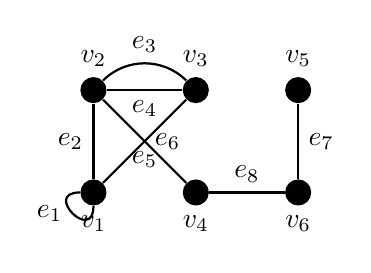
\begin{tikzpicture}[node distance = 1.3 cm]
                            \node (v_2) [solidNode, label=above:{$v_2$}] {};
                            \node (v_3) [solidNode, label=above:{$v_3$}, right of = v_2] {};
                            \node (v_1) [solidNode, label=below:{$v_1$}, below of = v_2] {};
                            \node (v_4) [solidNode, label=below:{$v_4$}, below of = v_3] {};
                            \node (v_5) [solidNode, label=above:{$v_5$}, right of = v_3] {};
                            \node (v_6) [solidNode, label=below:{$v_6$}, below of = v_5] {};
                            \draw [link] (v_2) -- node [left] {$e_2$} (v_1);
                            \draw [link] (v_2) -- node [below] {$e_5$} (v_4);
                            \draw [link] (v_1) to [out = 180, in = 270, looseness = 5] node [left] {$e_1$} (v_1);
                            \draw [link] (v_2) to [out = 45, in = 135] node [above] {$e_3$} (v_3);
                            \draw [link] (v_2) -- node [below] {$e_4$} (v_3);
                            \draw [link] (v_3) -- node [right] {$e_6$} (v_1);
                            \draw [link] (v_5) -- node [right] {$e_7$} (v_6);
                            \draw [link] (v_4) -- node [above] {$e_8$} (v_6);
                        \end{tikzpicture}
                    \end{figure}
                \end{example}

                \begin{definition}[Adjacent]
                    Two edges of a graph are \textbf{adjacent} if they have a common end, two vertices are \textbf{adjacent} if they are jointed by an edge.
                \end{definition}

                Saving a graph in computer program can be implemented in the following ways:
                \begin{itemize}
                    \item Adjacency matrix: $m \times n$ matrix, for $A[u, v] = 1$ if $(u, v) \in E$ and $A[u, v] = 0$ otherwise
                    \item Linked list: For every vertex $v$, there is a linked list containing all neighbors of $v$.
                \end{itemize}
                Assuming we are dealing with undirected graphs, $n$ is the number of vertices, $m$ is the number of edges, $n - 1 \le m \le n(n-1)/2$, $d_v$ is the number of neighbors of $v$ then
                \begin{table}[H]
                    \centering
                    \begin{tabular}{|c|c|c|}
                        \hline
                         & Matrix & Linked lists\\
                        \hline
                        memory usage & $O(n^2)$ & $O(m)$\\
                        \hline
                        time to check $(u, v) \in E$ & $O(1)$ & $O(d_u)$\\
                        \hline
                        time to list all neighbors of $v$ & $O(n)$ & $O(d_v)$\\
                        \hline
                    \end{tabular}
                \end{table}

            \paragraph{Subgraphs}
                \begin{definition}[Subgraph]
                    Given two graphs $G$ and $H$, $H$ is a \textbf{subgraph} of $G$ if $V(H)\subseteq V(G)$, $E(H)\subseteq E(G)$ and an edge has the same ends in $H$ as it does in $G$. Furthermore, if $E(H)\neq E(G)$ then $H$ is a proper subgraph.
                \end{definition}

                \begin{definition}[Vertex-induced, Edge-induced]
                    For a subset $V^\prime \subseteq V(G)$ we define an \textbf{vertex-induced} subgraph $G[V^\prime ]$ to be the subgraph with vertices $V^\prime$ and those edges of $G$ having both ends in $V^\prime$. The \textbf{edge-induced} subgraph $G[E^\prime ]$ has edges $E^\prime$ and those vertices of $G$ that are ends to edges in $E^\prime$.
                \end{definition}

                If we combine node-induced or edge-induced subgraphs $G(V^\prime )$ and $G(V - V^\prime )$, we cannot always get the entire graph.

                \begin{definition}[Degree]
                    Let $v\in V(G)$, then the \textbf{degree} of $v\in V(G)$ denote by $d_G(v)$ is defines to be the number of edges incident of $v$. Loops counted twice.
                \end{definition}

                \begin{theorem}
                    For any graph $G=(V, E)$
                    \begin{equation*}
                        \sum_{v\in V}d(v) = 2|E|
                    \end{equation*}
                \end{theorem}

                \begin{proof}
                    $\forall$ edge $e=uv$ with $u \neq v$, $e$ is counted once for $u$ and once for $v$, a total of two altogether. If $e=uu$, a loop, then it is counted twice for $u$.
                \end{proof}

                \begin{corollary}
                    Every graph has an even number of odd degree vertices.
                \end{corollary}

                \begin{proof}
                    \begin{equation*}
                        V = V_E\cup V_O \Rightarrow 
                        \sum_{v\in V}d(v) = \sum_{v\in V_E} d(v) + \sum_{v\in V_O}d(v) = 2|E|
                    \end{equation*}
                \end{proof}

            \paragraph{Special graphs}
                \begin{definition}[Complete Graph]
                    A \textbf{complete} graph $K_n (n \ge 1)$ is a simple graph with $n$ vertices and with exactly one edge between each pair of distinct vertices.
                \end{definition}

                \begin{definition}[Cycle Graph]
                    A \textbf{cycle} graph $C_n (n \ge 3)$ consists of $n$ vertices $v_1, ... v_n$ and $n$ edges $\{v_1, v_2\}, \{v_2, v_3\}, ... \{v_{n-1}, v_n\}$
                \end{definition}

                \begin{definition}[Wheel Graph]
                    A \textbf{wheel} graph $W_n (n \ge 3)$ is a simple graph obtains by adding one vertex to the cycle graph $C_n$, and connecting this new vertex to all vertices of $C_n$ 
                \end{definition}

                \begin{definition}[Bipartite Graph]
                    A simple graph is said to be \textbf{bipartite} if the vertex set can be expressed as the union of two disjoint non-empty subsets $V_1$ and $V_2$ such that every edges has one end in $V_1$ and another end in $V_2$
                \end{definition}

                \begin{example}
                    Here is an example for bipartite graph
                    \begin{figure}[H]
                        \centering
                        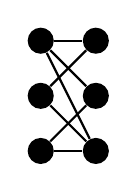
\begin{tikzpicture}[node distance = 0.7 cm]
                            \node (A) [solidNode] {};
                            \node (B) [solidNode, right of = A] {};
                            \node (C) [solidNode, below of = A] {};
                            \node (D) [solidNode, right of = C] {};
                            \node (E) [solidNode, below of = C] {};
                            \node (F) [solidNode, right of = E] {};
                            \draw [link] (A) -- (B);
                            \draw [link] (A) -- (D);
                            \draw [link] (C) -- (B);
                            \draw [link] (C) -- (F);
                            \draw [link] (E) -- (D);
                            \draw [link] (E) -- (F);
                            \draw [link] (A) -- (F);
                        \end{tikzpicture}
                    \end{figure}
                \end{example}

                \begin{definition}[Complete Bipartite Graph]
                    The \textbf{complete bipartite graph} $K_{mn}$ is the bipartite graph $V_1$ containing $m$ vertices and $V_2$ containing $n$ vertices such that each vertex in $V_1$ is adjacent to every vertex in $V_2$
                \end{definition}

                \begin{example}
                    Here is an example for $K_{53}$
                    \begin{figure}[H]
                        \centering
                        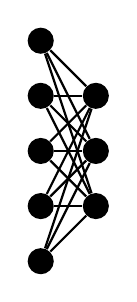
\begin{tikzpicture}[node distance = 0.7 cm]
                            \node (A) [solidNode] {};
                            \node (B) [solidNode, below of = A] {};
                            \node (C) [solidNode, below of = B] {};
                            \node (D) [solidNode, below of = C] {};
                            \node (E) [solidNode, below of = D] {};
                            \node (F) [solidNode, right of = B] {};
                            \node (G) [solidNode, right of = C] {};
                            \node (H) [solidNode, right of = D] {};
                            \draw [link] (A) -- (F);
                            \draw [link] (A) -- (G);
                            \draw [link] (A) -- (H);
                            \draw [link] (B) -- (F);
                            \draw [link] (B) -- (G);
                            \draw [link] (B) -- (H);
                            \draw [link] (C) -- (F);
                            \draw [link] (C) -- (G);
                            \draw [link] (C) -- (H);
                            \draw [link] (D) -- (F);
                            \draw [link] (D) -- (G);
                            \draw [link] (D) -- (H);
                            \draw [link] (E) -- (F);
                            \draw [link] (E) -- (G);
                            \draw [link] (E) -- (H);
                        \end{tikzpicture}
                    \end{figure}
                \end{example}

                \begin{theorem}
                    A graph $G$ is bipartite iff every cycle is even.
                \end{theorem}

                \begin{proof}
                    ($\Rightarrow$) If the graph $G$ is bipartite, by definition, the vertices of graph can be partition into two groups, that within the group there is no connection between vertices. Therefore, for each cycle, the odd index of vertices and even index of vertices has to be choose alternatively from each groups. Therefore the cycle has to be even.

                    ($\Leftarrow$) Prove by contradiction. A graph can be connected or not connected.

                    If $G$ is connected and has at least two vertices, for an arbitrary vertex $v\in V(G)$, we can calculate the minimum number of edges between the other vertices $v^\prime$ and $v$ (i.e., length, denoted by $l(v^\prime, v)$), for all the vertices that has odd length to $v$, assign them to set $V_1$, for the rest of vertices (and $v$), assign to set $V_2$. Assume that $G$ is not bipartite, which means there are at least one edge between distinct vertices in set $V_1$ or set $V_2$, without lost of generality, assume that edge is $uw$, $u, w\in V_1$. For all vertices in $V_1$ there is an odd length of path between the vertex and $v$, therefore, there exists an odd $l(u,v)$, and an odd $l(w-v)$. The length of cycle $l(u, w, v) = 1 + l(u, v) + l(w, v)$, which is an odd number, it contradict with the prerequisite that all cycles are even, which means the assumption that $G$ is not bipartite is incorrect, $G$ should be bipartite.

                    If $G$ is not connected. Then $G$ can be partition into a set of disjointed subgraphs which are connected with at least two vertices or contains only one vertex. For the component that has more that one vertices, we already proved that it has to be bipartite. For the subgraph $G_i \subset G, i = 1, 2, ..., n$, the vertices can be partition into $V_{i1} \in V(G_i)$ and $V_{i2} \in V(G_i)$, where $V_{i1} \cap V_{i2} = \emptyset$, the union of those subgraphs are bipartite too because $V_1 = \cup_{i=1}^n V_{i1} \in V(G)$ and $V_2 = \cup_{i=1}^n V_{i2} \in V(G)$ satisfied the condition of bipartite. For the subgraph that has one one vertices, those vertices can be assigned into either $V_1$ or $V_2$.
                \end{proof}

                \begin{example}
                    The following graph is bipartite, it only contains even cycles.
                    \begin{figure}[H]
                        \centering
                        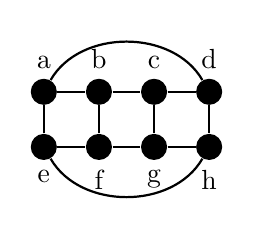
\begin{tikzpicture}[node distance=0.7 cm]
                            \node (a) [solidNode, label=above:{a}] {};
                            \node (b) [solidNode, label=above:{b}, right of = a] {};
                            \node (c) [solidNode, label=above:{c}, right of = b] {};
                            \node (d) [solidNode, label=above:{d}, right of = c] {};
                            \node (e) [solidNode, label=below:{e}, below of = a] {};
                            \node (f) [solidNode, label=below:{f}, below of = b] {};
                            \node (g) [solidNode, label=below:{g}, below of = c] {};
                            \node (h) [solidNode, label=below:{h}, below of = d] {};
                            \draw [link] (a) -- (b);
                            \draw [link] (b) -- (c);
                            \draw [link] (c) -- (d);
                            \draw [link] (a) -- (e);
                            \draw [link] (b) -- (f);
                            \draw [link] (c) -- (g);
                            \draw [link] (d) -- (h);
                            \draw [link] (e) -- (f);
                            \draw [link] (f) -- (g);
                            \draw [link] (g) -- (h);
                            \draw [link] (a) to [out = 60, in = 120, looseness = 1] (d);
                            \draw [link] (e) to [out = 300, in = 240, looseness = 1] (h);
                        \end{tikzpicture}
                    \end{figure}
                    We can rearrange the graph to be more clear as following\\
                    \begin{figure}[H]
                        \centering
                        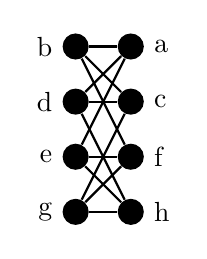
\begin{tikzpicture}[node distance=0.7 cm]
                            \node (a) [solidNode, label=right:{a}] {};
                            \node (b) [solidNode, label=left:{b}, left of=a] {};
                            \node (c) [solidNode, label=right:{c}, below of=a] {};
                            \node (d) [solidNode, label=left:{d}, below of=b] {};
                            \node (e) [solidNode, label=left:{e}, below of=d] {};
                            \node (f) [solidNode, label=right:{f}, below of=c] {};
                            \node (g) [solidNode, label=left:{g}, below of=e] {};
                            \node (h) [solidNode, label=right:{h}, below of=f] {};
                            \draw [link] (a) -- (b);
                            \draw [link] (b) -- (c);
                            \draw [link] (c) -- (d);
                            \draw [link] (a) -- (e);
                            \draw [link] (b) -- (f);
                            \draw [link] (c) -- (g);
                            \draw [link] (d) -- (h);
                            \draw [link] (e) -- (f);
                            \draw [link] (f) -- (g);
                            \draw [link] (g) -- (h);
                            \draw [link] (a) -- (d);
                            \draw [link] (e) -- (h);
                        \end{tikzpicture}
                    \end{figure}
                    The vertices of graph $G$ can be partition into two sets, $\{a, c, f, h\}$ and $\{b, d, e, g\}$
                \end{example}

                \begin{example}
                    The following graph is not bipartite

                    \begin{figure}[H]
                        \centering
                        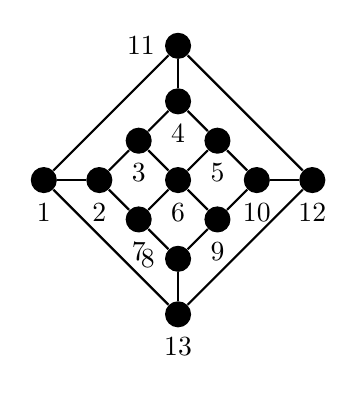
\begin{tikzpicture}[node distance=0.5 cm]
                            \node (11) [solidNode, label=left:{11}] {};
                            \node (4) [solidNode, label=below:{4}, below of=11, yshift=-0.205 cm] {};
                            \node (3) [solidNode, label=below:{3}, below of=4, xshift=-0.5 cm] {};
                            \node (5) [solidNode, label=below:{5}, below of=4, xshift=0.5 cm] {};
                            \node (1) [solidNode, label=below:{1}, below of=3, xshift=-1.205 cm] {};
                            \node (2) [solidNode, label=below:{2}, below of=3, xshift=-0.5 cm] {};
                            \node (6) [solidNode, label=below:{6}, below of=3, xshift=0.5 cm] {};
                            \node (10) [solidNode, label=below:{10}, below of=5, xshift=0.5 cm] {};
                            \node (12) [solidNode, label=below:{12}, below of=5, xshift=1.205 cm] {};
                            \node (7) [solidNode, label=below:{7}, below of=2, xshift=0.5 cm] {};
                            \node (8) [solidNode, label=left:{8}, below of=7, xshift=0.5 cm] {};
                            \node (9) [solidNode, label=below:{9}, below of=6, xshift=0.5 cm] {};
                            \node (13) [solidNode, label=below:{13}, below of=8, yshift=-0.205 cm] {};
                            \draw [link] (11) -- (1);
                            \draw [link] (11) -- (12);
                            \draw [link] (11) -- (4);
                            \draw [link] (4) -- (3);
                            \draw [link] (4) -- (5);
                            \draw [link] (3) -- (2);
                            \draw [link] (3) -- (6);
                            \draw [link] (5) -- (6);
                            \draw [link] (5) -- (10);
                            \draw [link] (1) -- (2);
                            \draw [link] (10) -- (12);
                            \draw [link] (2) -- (7);
                            \draw [link] (6) -- (7);
                            \draw [link] (6) -- (9);
                            \draw [link] (10) -- (9);
                            \draw [link] (7) -- (8);
                            \draw [link] (9) -- (8);
                            \draw [link] (8) -- (13);
                            \draw [link] (1) -- (13);
                            \draw [link] (12) -- (13);
                        \end{tikzpicture}
                    \end{figure}
                    The cycle $c=v_1v_{11}v_4v_3v_2$ have odd number of vertices.
                \end{example}

        \subsection{Walk, Path and Cycle}
            \paragraph{Walk, trail, path}
                \begin{definition}[walk]
                    A \textbf{walk} in a graph $G$ is a finite sequence $w=v_0e_1v_1e_2...e_kv_k$, where for each $e_i=v_{i-1}v_i$ the edge and its ends exists in $G$. We say that walk $v_0$ to $v_k$ on $(v_0, v_k)$-walk.
                \end{definition}

                \begin{example}
                    \begin{equation*}
                        w = v_2e_4v_3e_4v_2e_5v_3
                    \end{equation*}
                    is a walk, or $(v_2, v_3)$-walk
                \end{example}

                \begin{definition}[origin, terminal, internal, length]
                    For $(v_0, v_k)$-walk, The vertices $v_0$ and $v_k$ are called the \textbf{origin} and the \textbf{terminal} of the walk w, $v_1..v_{k-1}$ are called \textbf{internal} vertices. The integer $k$ is the \textbf{length} of the walk. Length of $w$ equals to the number of edges.
                \end{definition}

                We can create a reverse walk $w^{-1}$ by reversing $w$.
                \begin{equation*}
                    w^{-1} = v_ke_kv_{k-1}e_{k-1}...e_2v_1
                \end{equation*}
                (The reverse walk is guaranteed to exist because it is an undirected graph)

                Given two walks $w$ and $w'$ we can create a third walk denoted by $ww'$ by concatenating $w$ and $w'$. The new walk's origin is the same as terminal.

                \begin{definition}[trail]
                    A \textbf{trail} is a walk with no repeating edges. e.g., $v_3e_4v_2e_5v_3$
                \end{definition}

                \begin{definition}[path]
                    A \textbf{path} is a trail with no repeating vertices. e.g., $v_3e_4v_2$
                \end{definition}

                Paths $\subseteq$ Trails $\subseteq$ Walks

            \paragraph{Cycle}
                \begin{definition}[closed, cycle]
                    A path is \textbf{closed} if it has positive length and its origin and terminal are the same. e.g., $v_1e_2v_2e_4v_3e_3v_1$. A closed trail where origin and internal vertices are distinct is called a \textbf{cycle} (The only time a vertex is repeated is the origin and terminal)
                \end{definition}

                \begin{definition}[even cycle, odd cycle]
                    A cycle is \textbf{even} if it has a even number of edges otherwise it is \textbf{odd}.
                \end{definition}

                \begin{problem}
                    Prove that if $C_1$ and $C_2$ are cycles of a graph, then there exists cycles $K_1, K_2, ..., K_m$ such that $E(C_1)\Delta E(C_2) = E(K_1)\cup E(K_2) \cup...\cup E(K_m)$ and $E(K_i)\cap E(K_j)=\emptyset, \forall i \neq j$. (For set $X$ and $Y$, $X\Delta Y = (X-Y)\cup(Y-X)$, and is called the symmetric difference of $X$ and $Y$)
                \end{problem}

                \begin{proof}
                    Proof by constructing $K_1, K_2, ... K_m$. Denote 
                    \begin{align*}
                        C_1 & = v_{11}e_{11}v_{12}e_{12}v_{13}e_{13}...v_{1n}e_{1n}v_{11}\\
                        C_2 & = v_{21}e_{21}v_{22}e_{22}v_{23}e_{23}...v_{2k}e_{2k}v_{21}
                    \end{align*}
                    Assume both cycle start at the same vertice, $v_{11} = v_{12}$. (If there is no intersected vertex for $C_1$ and $C_2$, just simply set $K_1 = C_1$ and $K_2 = C_2$)\\
                    The following algorithm can give us all $K_j, j=1, 2, ... , m$ by constructing $E(C_1)\Delta E(C_2)$.  Also, the complexity is $O(mn)$, which makes the proof doable.\\
                    \begin{algorithm}[H]
                        \caption{Find $K_1, K_2, ... K_m$ by constructing $E(C_1)\Delta E(C_2)$}
                        \begin{algorithmic}[1]
                            \Require Graph $G$, cycle $C_1$ and $C_2$
                            \Ensure $K_1, K_2, ... K_m$
                            \State Initial, $K \gets \emptyset$, $j = 1$
                            \State Set temporary storage units, $v_o \gets v_{11}$, $v_t \gets \emptyset$
                            \For {$i = 1, 2, ..., n$}
                                \If {$e_{1i} \in C_2$}
                                    \If {$v_o \ne v_{1i}$}
                                        \State $v_t \gets v_{1i}$
                                        \State concatenate $(v_o, v_t)$-path $\subset C_1$ and $(v_o, v_t)$-path $\subset C_2$ to create a new $K_j$
                                        \State Append $K$ with $K_j$, $K \gets K \cup K_j$
                                        \State Reset temporary storage unit. $v_o \gets v_{1(i+1)}$ (or $v_{11}$ if $i = n$), $v_t \gets \emptyset$
                                    \Else
                                        \State $v_o \gets v_{1(i+1)}$ (or $v_{11}$ if $i = n$)
                                    \EndIf
                                \EndIf
                            \EndFor
                        \end{algorithmic}
                    \end{algorithm}
                    Now we prove that $K_i\cap K_j = \emptyset, \forall i \ne j$. For each $K_j$, it is defined by two $(v_o, v_t)$-paths in the algorithm. From the algorithm we know that all the edges in $(v_o, v_t)$-path in $C_1$ are not intersecting with $C_2$, because if the edge in $C_1$ is intersected with $C_2$, either we closed the cycle $K_j$ before the edge, or we updated $v_o$ after the edge (start a new $K_j$ after that edge). By definition of cycle, all the $(v_o, v_t)$-path that are subset of $C_1$ are not intersecting with each other, as well as all the $(v_o, v_t)$-path that are subset of $C_2$. Therefore, $K_i\cap K_j = \emptyset, \forall i \ne j$.
                \end{proof}

        \subsection{Some warm-up algorithms}
            \paragraph{Component}
                \begin{definition}[connected vertices]
                    Two vertices $u$ and $v$ in a graph are said to be \textbf{connected} if there is a path between $u$ and $v$.
                \end{definition}

                \begin{definition}[component]
                    Connectivity between vertices is an equivalence relation on $V(G)$, if $V_1, ... V_k$ are the corresponding equivalent classes then $G[V_1]...G[V_k]$ are \textbf{components} of G. If graph has only one component, then we say the graph is connected. A graph is connected iff every pair of vertices in G are connected, i.e., there exists a path between every pair of vertices.
                \end{definition}

                The following algorithm finds components in a given graph $G = (V, E)$.

                \begin{algorithm}[H]
                    \centering
                    \caption{Find components}
                    \begin{algorithmic}[1]
                        \State Let $Q$ be the set of components
                        \For {$i \in V$}
                            \State $Q \gets \{i\}$
                        \EndFor
                        \For {$e = (i, j) \in E$}
                            \For {$p \in Q$}
                                \For {$q \in Q$}
                                    \If {$i \in p$ and $j \in q$}
                                        \State $Q \gets Q \setminus p \setminus q \cup (p \cup Q)$
                                    \EndIf
                                \EndFor
                            \EndFor
                        \EndFor
                        \State \Return Q
                    \end{algorithmic}
                \end{algorithm}

                We will revisit this procedure when we discuss the subtour elimination constraints for TSP. Such procedure can be improved by introducing disjoint-set forest.

            \paragraph{Cycle detection}
                The following algorithm is for connected graph, if the graph is not connected, run the algorithm for each component until cycle is detected or all the components have been calculated. Since the complexity for running in connected graph is $O(n + m)$, $n$ as the number of vertices/nodes, and $m$ as the number of edges/arcs, the running time of disconnected graph is the \textbf{summation} of running time in each component, where each component is connected. Therefore the complexity is the same in disconnected graph as in connected graph.

                The main idea is starting with arbitrary vertex/node, using DFS or BFS to search on the graph try to revisit the vertex/node we start with. If succeed, a cycle is detected, otherwise if all the vertices/nodes has been visited, then no cycle exists. And in linked-list representation, the complexity is $O(|V| + |E|)$, i.e. $O(n + m)$. However, there is slightly different in undirected graph and directed graph, for undirected graph needs at least three vertices to form a cycle while directed graph needs at least two.

                Here is the detail algorithm (DFS) for undirected graph:
                \begin{algorithm}[H]
                    \caption{Main algorithm}
                    \begin{algorithmic}[1]
                        \State For all nodes, labeled as ``unvisited''
                        \State Arbitrary choose a vertex $v$, add a dummy vertex $w$, add a dummy edge $(w, v)$, label $w$ as ``visited''
                        \State run $DFS(w, v)$
                        \State Remove dummy vertex $w$ and dummy edge $(w, v)$
                        \If {$DFS(w, v)$ returns ``Cycle is found''}
                            \State \Return ``Cycle is found''
                        \Else
                            \State \Return ``No cycle detected''
                        \EndIf
                    \end{algorithmic}
                \end{algorithm}

                \begin{algorithm}[H]
                    \caption{DFS(w, v)}
                    \begin{algorithmic}[1]
                        \State Label $v$ as ``visited''
                        \If {number of $v$ 's neighbor is 1}
                            \State \Return null
                        \Else
                            \For {all neighbor $u$ in linked-list of $v$ excepts $w$}
                                \If {$u$ is labeled as ``visited''} 
                                    \State \Return ``Cycle is found'' 
                                \Else
                                    \State run $DFS(v, u)$
                                \EndIf
                            \EndFor
                        \EndIf
                    \end{algorithmic}
                \end{algorithm}

                Now check the complexity. Denote $v\in N$ as a node in graph $G$, total number of nodes denoted by $n$, denote $d_v$ as number of neighbors of node $v$. The complexity of $DFS(w, v)$ is $O(d_v)$ for each node $v$ it visited (it should be $O(v)$ because we need $O(1)$ to check if a node is $w$), each node can only be visited, by ``visited'' it means $DFS(w, v)$ is executed, at most once, which is controlled by the ``visited'' label. The total complexity is $O(n + \sum_{v\in N} d_v) = O(n + m)$

            \paragraph{Test Bipartiteness}
                We have proved that a bipartite graph only has even cycles, and the graph with only even cycles are bipartite graph, however, that is not very convenient to test if a graph is bipartite because it needs to enumerate all cycles.

                The other idea to test bipartiteness is try to color the vertices of the graph, if it can be 2-colored, then the graph is bipartite, otherwise it is not.

                The following is the algorithm (using BFS)
                \begin{algorithm}[H]
                    \caption{Test Bipartiteness}
                    \begin{algorithmic}[1]
                        \State Initialize, $head \gets 1$, $tail \gets 1$, $queue[1] \gets s$, mark all vertices as ``unvisited''
                        \State Mark $s$ as ``visited''
                        \State $color[s] \gets 0$
                        \While {$head \ge tail$}
                            \State $v \gets queue[tail]$, $tail \gets tail + 1$
                            \For {$\forall u \in d_v$}
                                \If {$u$ is ``unvisited''}
                                    \State $head \gets head + 1$, $queue[head] = u$
                                    \State Mark $u$ as ``visited''
                                    \State $color[u] \gets 1 - color[v]$
                                \Else
                                    \If {$color[u] == color[v]$}
                                        \Return False
                                    \EndIf
                                \EndIf
                            \EndFor
                        \EndWhile
                        \Return True
                    \end{algorithmic}
                \end{algorithm}

            \paragraph{Bridge}
                \begin{definition}[Tree Edge, Cross Edge, Vertical Edge]
                    Given a graph $G = (V, E)$ and a rooted tree $T$ in $G$, edge in $G$ can be classified by three types:
                    \begin{itemize}
                        \item Tree edges: edge in $T$
                        \item Cross edges: $(u, v)$, $u$ and $v$ do not have an ancestor-descendant relation
                        \item Vertical edges: $(u, v)$, $u$ is an ancestor of $v$, or $v$ is an ancestor of $u$
                    \end{itemize}

                    \begin{figure}[H]
                        \centering
                        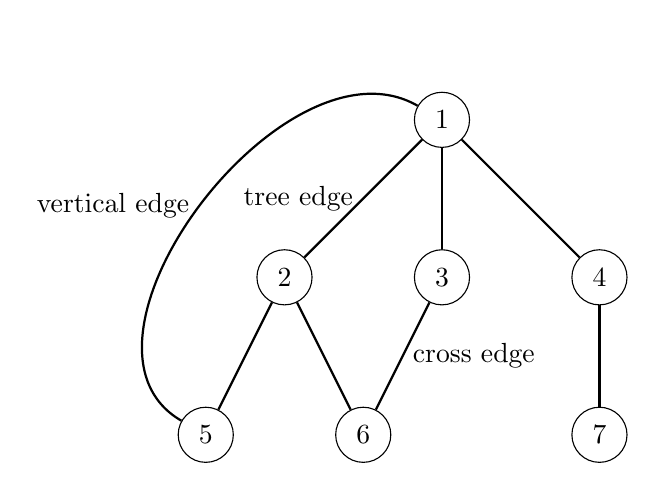
\begin{tikzpicture}[node distance=2 cm]
                            \node (1) [circleNode] {1};
                            \node (2) [circleNode, below of=1, xshift = -2 cm] {2};
                            \node (3) [circleNode, below of=1] {3};
                            \node (4) [circleNode, below of=1, xshift = 2 cm] {4};
                            \node (5) [circleNode, below of=2, xshift = -1 cm] {5};
                            \node (6) [circleNode, below of=2, xshift = 1 cm] {6};
                            \node (7) [circleNode, below of=4] {7};
                            \draw [link] (1) -- node [left] {tree edge} (2);
                            \draw [link] (1) -- (3);
                            \draw [link] (1) -- (4);
                            \draw [link] (2) -- (5);
                            \draw [link] (2) -- (6);
                            \draw [link] (4) -- (7);
                            \draw [link] (3) -- node [right] {cross edge} (6);
                            \draw [link] (1) to [out = 150, in = 150] node [left] {vertical edge} (5);
                        \end{tikzpicture}
                    \end{figure}
                \end{definition}

                In a BFS tree $T$ of a graph $G$, there can not be vertical edges, there cannot be cross edges $(u, v)$ with $u$ and $v$ 2 levels apart. (Cross edge at most 1 level apart)

                In a DFS tree $T$ of a graph $G$, there can not be cross edges, there can only be tree edges and vertical edges.

                \begin{definition}[bridge]
                    Given a connected graph $G=(V, E)$, an edge $e \in E$ is called a \textbf{bridge} if the graph $G=(V, E\setminus \{e\})$ is disconnected.
                \end{definition}

                The idea to find bridge is through a DFS tree. Notice that there are only tree edges and vertical edges in DFS tree. Vertical edges are not bridges, a tree edge $(u, v)$ is not a bridge if some vertical edge jumping from below $u$ to above $v$. Other tree edges are bridges.

                Define $level(v)$ as the level of vertex $v$ in DFS tree. $T_v$ as the sub tree rooted at $v$, $h(v)$ as the smallest level that can be reached using a vertical edge from vertices in $T_v$. $(parent(u), u)$ is a bridge if $h(u) \ge level(u)$. The algorithm is as following:
                \begin{algorithm}[H]
                    \caption{FindBridge(G)}
                    \begin{algorithmic}[1]
                        \State Mark all vertices as ``unvisited''
                        \For {$v \in V$}
                            \If {$v$ is ``unvisited''}
                                \State $level(v) \gets 0$
                                \State \texttt{RecursiveDFS(v)}
                            \EndIf
                        \EndFor
                    \end{algorithmic}
                \end{algorithm}

                \begin{algorithm}[H]
                    \caption{RecursiveDFS(v)}
                    \begin{algorithmic}[1]
                        \State mark $v$ as ``visited''
                        \State $h(v) \gets \infty$
                        \For {$u \in d_v$}
                            \If {$u$ is ``unvisited''}
                                \State $level(u) \gets level(v) + 1$
                                \State \texttt{RecursiveDFS(u)}
                                \If {$h(u) \ge level(u)$}
                                    \State $(u, v)$ is a bridge
                                \EndIf
                                \If {$h(u) < h(v)$}
                                    \State $h(v) \gets h(u)$
                                \EndIf
                            \Else
                                \If {$level(u) < level(v) - 1$ and $level(u) < h(v)$}
                                    \State $h(v) \gets level(u)$
                                \EndIf
                            \EndIf
                        \EndFor
                    \end{algorithmic}
                \end{algorithm}

    \section{Matching}
        \subsection{Matching}
            \begin{definition}[matching, M-saturated, M-unsaturated]
                Let $G = (V, E)$ be a graph, a \textbf{matching} is a subset of edges $M \subseteq E$ such that no two elements of $M$ are adjacent. The two ends of an edge in $M$ are said to be \textbf{matched} under $M$. A matching $M$ saturates a vertex $v$, and $v$ is said to be \textbf{M-saturated}, if some edge of $M$ is incident with $v$. Otherwise, $v$ is \textbf{M-unsaturated}.
            \end{definition}

            \begin{definition}[perfect matching, maximum matching]
                If every vertex of $G$ is M-saturated, then the matching is said to be \textbf{perfect matching}, for perfect matching, we have $|M| = \frac{|V(G)|}{2}$. $M$ is a \textbf{maximum matching} if $G$ has no matching $M^\prime$ with $|M^\prime| > |M|$. Every perfect matching is maximum. The maximum matching does not necessarily to be perfect. Perfect matching and maximum matching may not be unique.
            \end{definition}

            \begin{definition}[M-alternating]
                An \textbf{M-alternating} path in $G$ is a path whose edges are alternately in $E\setminus M$ and $M$.
            \end{definition}

            \begin{definition}[M-augmenting]
                An \textbf{M-augmenting} path in $G$ is an $M$-alternating path whose origin and terminus are $M$-unsaturated.
            \end{definition}

            \begin{lemma}
                Every augmenting path $P$ has property that let $M^\prime = P\Delta M = (M \cup P) \setminus (M \cap P)$ then $M^\prime$ contains one more edge then $M$
            \end{lemma}

            The following path is an $M$-augmenting path
            \begin{figure}[H]
                \centering
                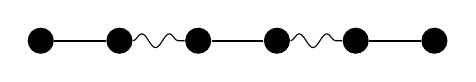
\begin{tikzpicture}
                    \node (0) [solidNode] {};
                    \node (1) [solidNode, right of=0] {};
                    \node (2) [solidNode, right of=1] {};
                    \node (3) [solidNode, right of=2] {};
                    \node (4) [solidNode, right of=3] {};
                    \node (5) [solidNode, right of=4] {};
                    \draw (0) [link] -- (1);
                    \draw (1) [matchedLink] -- (2);
                    \draw (2) [link] -- (3);
                    \draw (3) [matchedLink] -- (4);
                    \draw (4) [link] -- (5);
                \end{tikzpicture}
            \end{figure}

            The following path is $M^\prime = P\Delta M (M \cup P) \setminus (M \cap P)$ and all the vertices are $M$-saturated.

            \begin{figure}[H]
                \centering
                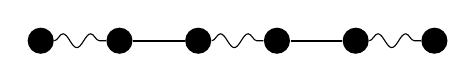
\begin{tikzpicture}
                    \node (0) [solidNode] {};
                    \node (1) [solidNode, right of=0] {};
                    \node (2) [solidNode, right of=1] {};
                    \node (3) [solidNode, right of=2] {};
                    \node (4) [solidNode, right of=3] {};
                    \node (5) [solidNode, right of=4] {};
                    \draw (0) [matchedLink] -- (1);
                    \draw (1) [link] -- (2);
                    \draw (2) [matchedLink] -- (3);
                    \draw (3) [link] -- (4);
                    \draw (4) [matchedLink] -- (5);
                \end{tikzpicture}
            \end{figure}

            \begin{theorem}[Berge, 1957]
                A matching $M$ in a graph $G$ is maximum iff $G$ has no M-augmenting path.
            \end{theorem}

            \begin{proof}
                ($\Rightarrow$) It is clear that if $M$ is maximum, it has no augmenting paths since otherwise by problem claim we can increase by one.

                ($\Leftarrow$) Suppose $M$ is not maximum and let $M^\prime$ be a bigger matching. Let $A = M \Delta M^\prime$ now no vertex of $G$ is incident to more than two members of $A$. For otherwise either two members of $M$ or two members of $M^\prime$ would be adjacent. Contradict the definition of matching. It follows that every component of the edges incident subgraph $G[A]$ is either an even cycle with edge augmenting in $M\Delta M^\prime$ or else $A$ path with edges alternating between $M$ and $M^\prime$.

                Since $|M^\prime| \ge |M|$ then the even cycle cannot help because exchanging $M$ and $M^\prime$ will have same cardinality.

                The path case implies that $p$ is alternating in $M$ and since $|M^\prime| > |M|$ the end arc exposed so that $p$ is augmenting.
            \end{proof}

            \begin{definition}[Vertex-cover]
                The \textbf{vertex-cover} is a subset of vertices $X$ such that every edge of $G$ is incident to some member of $X$.
            \end{definition}

            \begin{lemma}
                The cardinality of any matching is less than or equal to the cardinality of any vertex cover.
            \end{lemma}

            \begin{proof}
                Consider any matching. Any vertex cover must have nodes that at least incident to the edges in the matching. Since all the edges in the matching are disjointed, so for a single node can at most cover one edge in the matching. If the matching is not perfect, for the edges that not in the tree, they may or may not be possible to be covered by the nodes incident to the edges in the matching, with an easy triangle graph example, we can prove this lemma.
            \end{proof}

            \begin{theorem}[K\"onig Theorem]
                If $G$ is bipartite, the cardinality of the maximum matching is equal to the cardinality of the minimum vertex cover.
            \end{theorem}

            \begin{proof}
                Let $G$ be a bipartite graph, $G = (V, E)$ where $V = X\cup Y$ as $X$ and $Y$ are two disjointed sets of vertices. Let $M$ be a maximum matching on $G$. For each edge in $M$, denoted by $e_i = a_ib_i$ where $e_i \in M$, $a_i \in A$ and $b_i \in B$ and $A = \{a_i: e_i \in M\} \subseteq X$, and $B = \{b_i: e_i \in M\} \subseteq Y$. Therefore, we can partition $X$ by $A$ and $U = X\setminus A$, partition $Y$ by $B$ and $W = Y\setminus B$.

                We can further partition the matching $M$ into $M_1$ and $M_2$. For all the edges in $M_1$ can be included into an $M$-alternating path starts from a vertex in $U$ (which includes the edges directly linked to vertices in $U$), and $M_2 = M \setminus M_1$. For edges in $M_1$, we take the ends of edges in $B$ in the vertex cover, denoted by $B_1$, take the ends of edges in $A$ as a subset denoted by $A_1 \subseteq A$. For the edges in $M_2$, we take the ends of edges in $A$ in the vertex cover, denoted by $A_2$, and the ends of edges in $B$ as a subset denoted by $B_2 \subseteq B$. 

                We claim that all the vertices in $U$ can only be connected to vertices in $B_1$ and vertices in $W$ can only be connected to vertices in $A_2$.

                $U \subset X$ connects to vertices in $B_1$ by definition. If vertices in $W \subset Y$ is connected to vertices in $A_1$, then we will have $M$-augmenting path which is contradicted to the assumption that $M$ is maximum matching.
            \end{proof}

            The following is an example. Where the edge in the matching that accessible from members of $U = \{1, 2\}$ in an $M$-alternating path is edge $3a, 4b, 5c, 6d$.

            \begin{figure}[H]
                \centering
                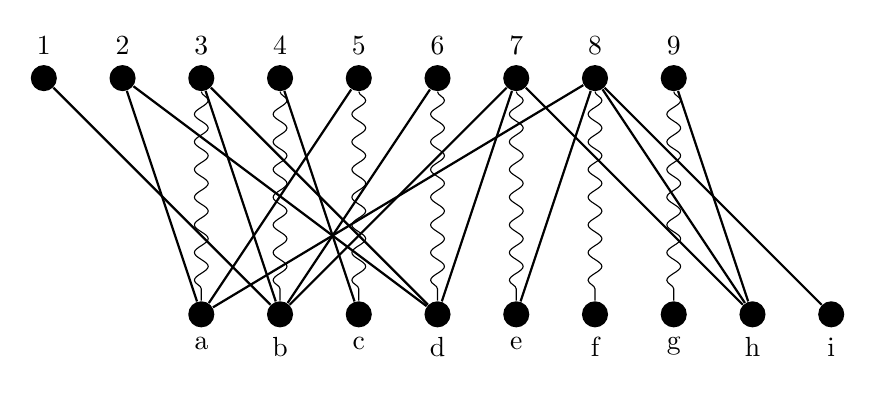
\begin{tikzpicture}
                    \node (1) [solidNode, label=above:{1}] {};
                    \node (2) [solidNode, right of = 1, label=above:{2}] {};
                    \node (3) [solidNode, right of = 2, label=above:{3}] {};
                    \node (4) [solidNode, right of = 3, label=above:{4}] {};
                    \node (5) [solidNode, right of = 4, label=above:{5}] {};
                    \node (6) [solidNode, right of = 5, label=above:{6}] {};
                    \node (7) [solidNode, right of = 6, label=above:{7}] {};
                    \node (8) [solidNode, right of = 7, label=above:{8}] {};
                    \node (9) [solidNode, right of = 8, label=above:{9}] {};
                    \node (a) [solidNode, below of = 3, yshift=-2 cm, label=below:{a}] {};
                    \node (b) [solidNode, right of = a, label=below:{b}] {};
                    \node (c) [solidNode, right of = b, label=below:{c}] {};
                    \node (d) [solidNode, right of = c, label=below:{d}] {};
                    \node (e) [solidNode, right of = d, label=below:{e}] {};
                    \node (f) [solidNode, right of = e, label=below:{f}] {};
                    \node (g) [solidNode, right of = f, label=below:{g}] {};
                    \node (h) [solidNode, right of = g, label=below:{h}] {};
                    \node (i) [solidNode, right of = h, label=below:{i}] {};
                    \draw [matchedLink] (3) -- (a);
                    \draw [matchedLink] (4) -- (b);
                    \draw [matchedLink] (5) -- (c);
                    \draw [matchedLink] (6) -- (d);
                    \draw [matchedLink] (7) -- (e);
                    \draw [matchedLink] (8) -- (f);
                    \draw [matchedLink] (9) -- (g);
                    \draw [link] (1) -- (b);
                    \draw [link] (2) -- (a);
                    \draw [link] (8) -- (i);
                    \draw [link] (8) -- (h);
                    \draw [link] (3) -- (b);
                    \draw [link] (3) -- (d);
                    \draw [link] (2) -- (d);
                    \draw [link] (4) -- (c);
                    \draw [link] (5) -- (a);
                    \draw [link] (6) -- (b);
                    \draw [link] (7) -- (b);
                    \draw [link] (7) -- (d);
                    \draw [link] (7) -- (h);
                    \draw [link] (8) -- (e);
                    \draw [link] (8) -- (a);
                    \draw [link] (9) -- (h);
                \end{tikzpicture}
            \end{figure}

            In which $U = \{1, 2\}$, $M_1 = \{3a, 4b, 5c, 6d\}$. $U = \{1, 2,\}, A_1 = \{3, 4, 5, 6\}, A_2 = \{7, 8, 9\}, W=\{h, i\}, B_1 = \{a, b, c, d\}, B_2 = \{e, f, g\}$. The vertex cover is $\{a, b, c, d, 7, 8, 9\}$.

            The above theorem does not apply to non-bipartite graph. The following is an example
            \begin{figure}[H]
                \centering
                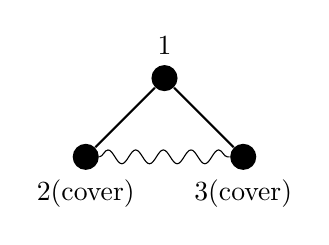
\begin{tikzpicture}
                    \node (1) [solidNode, label=above:{1}] {};
                    \node (2) [solidNode, below of = 1, xshift = -1 cm, label=below:{2(cover)}] {};
                    \node (3) [solidNode, below of = 1, xshift = 1 cm, label=below:{3(cover)}] {};
                    \draw [matchedLink] (2) -- (3);
                    \draw [link] (1) -- (2);
                    \draw [link] (1) -- (3);
                \end{tikzpicture}
            \end{figure}

            The maximum matching has one edge, where the minimum cover has two vertices.

        \subsection{Blossom Algorithm}
            First, for the bipartite graphs, there is no odd cycles in the graph, the maximum matching can be derived by repeatedly extend the existing augmenting paths. For the non-bipartite algorithm, we use the Blossom algorithm to find maximum matching.

            \paragraph{Blossom}
            A blossom is a set of nodes and edges starting at an unsaturated vertex, with a stem of even number of edges, and link to an odd cycle of edges. 

            \begin{figure}[H]
                \centering
                \includegraphics[width=0.4\textwidth]{"../../image/blossom"}
                \caption{An example of blossom}
            \end{figure}

            \paragraph{Pseudo codes}
                \begin{algorithm}
                    \centering
                    \caption{Blossom algorithm}
                    \begin{algorithmic}
                        \State Let $F$ be the set of unsaturated nodes
                        \While {$F \neq \emptyset$}
                            \State Let $r \in F$ be an unsaturated node
                            \State queue.push($r$)
                            \State $T \gets \emptyset$
                            \State $T$.add($r$)
                            \While {queue $\neq \emptyset$}
                                \State $v \gets$ queue.pop()
                                \For {All neighbor $w$ of $v$}
                                    \If {$w \notin T$ and $w$ is saturated}
                                        \State $T$.add(w)
                                        \State $T$.add(mate(w)), mate(w) is another neighbor of $w$
                                        \State queue.push(mate(w))
                                    \ElsIf {$w \in T$ and odd cycle detected}
                                        \State Contract cycle
                                    \ElsIf {$w \in F$}
                                        \State Expand all contract cycles
                                        \State Reconstruct augmenting path
                                        \State Augment path by inverting edges
                                    \EndIf
                                \EndFor
                            \EndWhile
                        \EndWhile
                    \end{algorithmic}
                \end{algorithm}    

    \section{Maximum Flow Problem}
        \subsection{Maximum Flow Problem}
            Let $D=(V, A)$ be a strict digraph with distinguished vertices $s$ and $t$. We call $s$ the source and $t$ the sink, let $u=\{u_e: e\in A\}$ be a nonnegative integer-valued capacity function defined on the arcs of $D$. The maximum flow problem on $(D, s, t, u)$ is the following Linear program.
            \begin{align*}
                \max \quad & v\\
                \text{s.t.} \quad & \sum_{h(e)=i}x_e - \sum_{t(e) = i} x_e = \begin{cases}
                    -v, \quad \text{if } i = s\\
                    v, \quad \text{if } i = t \\
                    0, \quad \text{otherwise}
                \end{cases}\\
                & 0\le x_e \le u_e, \quad \forall e\in A
            \end{align*}
            We think of $x_e$ as being the flow on arc $e$. Constraint says that for $i \neq s, t$ the flow into a vertex has to be equal to the flow out of vertex. That is, flow is conceded at vertex $i$ for $i=s$ and for $i=t$ the net flow in the entire digraph must be equal to $v$. A $\mathbf{x_e}$ that satisfied the above constraints is an $(s,t)$-flow of value $v$. If in addition it satisfies the bounding constraints, then it is a feasible $(s,t)$-flow. A feasible $(s,t)$-flow that has maximum $v$ is optimal on maximum.

            \begin{theorem}
                For $S \subseteq V$ we define $(S, \bar{S})$ to be a $(s, t)$-cut if $s\in S$ and $t\in \bar{S}=V-S$, the capacity of the cut, denoted $u(S, \bar{S})$ as $\sum \{u_e: e\in \delta^-(S)\}$ where $\delta^-(S) = \{e\in A: t(e) \in S \text{ and } h(e) \in \bar{S}\}$
            \end{theorem}

            \begin{example}
                For the following graph:
                \begin{figure}[H]
                    \centering
                    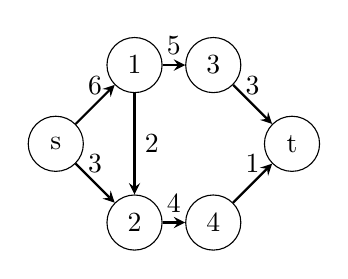
\begin{tikzpicture}[node distance = 1 cm]
                        \node (1) [circleNode] {1};
                        \node (3) [circleNode, right of=1] {3};
                        \node (s) [circleNode, below of=1, xshift = -1 cm] {s};
                        \node (2) [circleNode, below of=s, xshift = 1 cm] {2};
                        \node (t) [circleNode, below of=3, xshift = 1 cm] {t};
                        \node (4) [circleNode, below of=t, xshift = -1 cm] {4};
                        \draw [arrow] (s) -- node [above] {6} (1);
                        \draw [arrow] (s) -- node [above] {3} (2);
                        \draw [arrow] (1) -- node [right] {2} (2);
                        \draw [arrow] (1) -- node [above] {5} (3);
                        \draw [arrow] (2) -- node [above] {4} (4);
                        \draw [arrow] (3) -- node [above] {3} (t);
                        \draw [arrow] (4) -- node [above] {1} (t);
                    \end{tikzpicture}
                \end{figure}
                Let $S = \{1, 2, 3, s\}$, $\bar{S} = \{4, t\}$\\
                then $\delta^-(S) = \{(2, 4), (3, t)\} \Rightarrow u(S, \bar{S}) = 7$
            \end{example}

            \begin{definition}
                If $(S, \bar{S})$ has minimum capacity of all $(s,t)$-cuts, then it is called \textbf{minimum cut}.
            \end{definition}

            \begin{definition}
                Let $\delta^+(S) = \delta^-(V-S)$
            \end{definition}

            \begin{example}
                \begin{figure}[H]
                    \centering
                    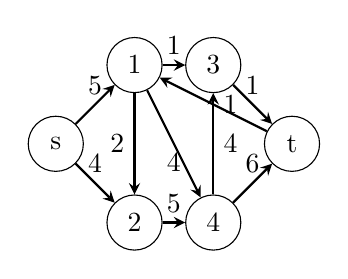
\begin{tikzpicture}[node distance = 1 cm]
                        \node (1) [circleNode] {1};
                        \node (3) [circleNode, right of=1] {3};
                        \node (s) [circleNode, below of=1, xshift = -1 cm] {s};
                        \node (2) [circleNode, below of=s, xshift = 1 cm] {2};
                        \node (t) [circleNode, below of=3, xshift = 1 cm] {t};
                        \node (4) [circleNode, below of=t, xshift = -1 cm] {4};
                        \draw [arrow] (s) -- node [above] {5} (1);
                        \draw [arrow] (s) -- node [above] {4} (2);
                        \draw [arrow] (1) -- node [left] {2} (2);
                        \draw [arrow] (1) -- node [above] {1} (3);
                        \draw [arrow] (1) -- node [below] {4} (4);
                        \draw [arrow] (2) -- node [above] {5} (4);
                        \draw [arrow] (4) -- node [right] {4} (3);
                        \draw [arrow] (3) -- node [above] {1} (t);
                        \draw [arrow] (4) -- node [above] {6} (t);
                        \draw [arrow] (t) -- node [right] {1} (1);
                    \end{tikzpicture}
                \end{figure}

                Let $S = \{s, 1, 2, 3\}$, $\bar{S} = \{4, t\}$, $u(S, \bar{S}) = u_{14} + u_{24} + u_{3t} = 10$, $\delta^-(S) = \{(1, 4), (2, 4), (3, t)\}$, $\delta^+(S) = \{(4, 3), (t, 1)\}$
            \end{example}

            \begin{lemma}
                If $x$ is a $(s, t)$ flow of value $v$ and $(S, \bar{S})$ is a $(s, t)$-cut, then
                \begin{equation*}
                    v = \sum_{e\in \delta^-(S)} x_e - \sum_{e\in \delta^+(S)} x_e
                \end{equation*}
            \end{lemma}

            \begin{proof}
                Summing the first set of constraints over the vertices of $S$,
                \begin{equation*}
                    \sum_{i\in S} (\sum_{h(e) = i}x_e - \sum_{t(e) = i}x_e) = -v
                \end{equation*}
                Now for an arc $e$ with both ends in $S$, $x_e$ will occur twice once with a positive and once with negative so they cancel and the above sum is reduced to
                \begin{equation*}
                    \sum_{e\in \delta^+(S)}x_e - \sum_{e \in \delta^-(S)}x_e = -v
                \end{equation*}
            \end{proof}

            Flow is the prime variable, capacity is the dual variable.

            \begin{corollary}
                If $x$ is a feasible flow of value $v$, and $(S, \bar{S})$ is an $(s, t)$-cut, then
                \begin{equation*}
                    v \le u(S, \bar{S}) \quad \text{(Weak duality)}
                \end{equation*}
            \end{corollary}

            \begin{definition}
                Define an arc $e$ to be \textbf{saturated} if $x_e = u_e$, and to be \textbf{flowless} if $x_e = 0$
            \end{definition}

            \begin{corollary}
                Let $x$ be a feasible flow and $(S, \bar{S})$ be a $(s, t)$-cut, if $\forall e\in \delta^-(S)$ is saturated, and $\forall e\in \delta^+(S)$ is flowless, then $x$ is a maximum flow and $(S, \bar{S})$ is a minimum cut. (Strong duality)
            \end{corollary}

            \begin{proof}
                If every arc of $\delta^-(S)$ is saturated then
                \begin{equation*}
                    \sum_{e\in \delta^-(S)}x_e = \sum_{e\in \delta^-(S)}u_e
                \end{equation*}
                If every arc of $\delta^+(S)$ is flowless then
                \begin{equation*}
                    \sum_{e\in \delta^+(S)}x_e = 0
                \end{equation*}
                $\Rightarrow$ $x$ is as large as it can get when as $u(S, \bar{S})$ is as small as it can get.
            \end{proof}

        \subsection{Prime and Dual of Maximum Network Flow Problem}
            The LP of maximum flow can be modeled as following, WLOG, we let $s = v_1 \in V, t = v_{|V|} \in V$.
            \begin{align*}
                \max \quad & f = \left[\begin{matrix}0 & 0 & \cdots & 0 & 1\end{matrix}\right]\left[\begin{matrix}\mathbf{x} \\ f\end{matrix}\right]\\
                \text{s.t.} \quad & \left[\begin{matrix}\mathbf{A} & \mathbf{F}\end{matrix}\right]\left[\begin{matrix}\mathbf{x}\\ f\end{matrix}\right] = \mathbf{0}\\
                & \mathbf{Ix} \le \mathbf{u}\\
                & \left[\begin{matrix}\mathbf{x}\\ f\end{matrix}\right] \ge 0
            \end{align*}

            In which $\mathbf{A}$ is the vertex-arc incident matrix and $\mathbf{F}$ is a column vector where the first row is -1, last row is 1 and all other rows are 0s, which is because we denote the first vertex as source $s$ and the last vertex as the sink $t$. $\mathbf{u}$ is the column vector of upper bound of each arcs.
            \begin{align*}
                \mathbf{A} &= \mathbf{A}_{|E|\times |V|} = [a_{ij}], \text{ where } a_{ij} = \begin{cases}
                    1, \quad \text{if $v_i = h(e_j)$} \\
                    -1, \quad \text{if $v_i = t(e_j)$} \\
                    0, \quad \text{otherwise}
                \end{cases}\\
                \mathbf{F} &= \left[\begin{matrix}-1 & \cdots & 0 & \cdots & 1\end{matrix}\right]^\top \\
                \mathbf{u} &= \left[\begin{matrix}u_1 & u_2 & \cdots & u_{|E|}\end{matrix}\right]^\top
            \end{align*}

            Then, we take the dual of LP
            \begin{align*}
                \min \quad & \mathbf{u}\mathbf{w_E} \\
                \text{s.t.} \quad & \left[\begin{matrix}
                    \mathbf{w_V} & \mathbf{w_E}
                \end{matrix}\right]\left[\begin{matrix}
                    \mathbf{A} \\ \mathbf{I}
                \end{matrix}\right] \ge 0 \\
                & \left[\begin{matrix}
                    \mathbf{w_V} & \mathbf{w_E}
                \end{matrix}\right]\left[\begin{matrix}
                    \mathbf{F} \\\mathbf{0}
                \end{matrix}\right] = 1\\
                & \mathbf{w_V} \quad \text{unrestricted} \\
                & \mathbf{w_E} \ge \mathbf{0}
            \end{align*}

            In which $\mathbf{w_V}$ is ``whether or not'' vertex $v$ is in $S$ where $(S, \bar{S})$ represents a cut, $\mathbf{w_E}$ is ``whether or not'' an arc in in $\delta^+(S)$. $\mathbf{u}, \mathbf{E}, \mathbf{F}$ have the same meaning as in prime.
            \begin{align*}
                \mathbf{w_V} &= \left[\begin{matrix}w_1 & w_2 & \cdots & w_{|V|}\end{matrix}\right]^\top \\
                \mathbf{w_E} &= \left[\begin{matrix}w_{|V| + 1} & w_{|V| + 2} & \cdots & w_{|V| + |E|}\end{matrix}\right]^\top
            \end{align*}

            To make it more clear, it can be rewritten as following
            \begin{align*}
                \min \quad & \sum_{e \in E} u_ew_e\\
                \text{s.t.} \quad & w_i - w_j + w_{|V| + e} \ge 0, \forall e = (i, j) \in E\\
                & -w_1 + w_{|V|} = 1\\
                & \mathbf{w_V} \quad \text{unrestricted} \\
                & \mathbf{w_E} \ge \mathbf{0}
            \end{align*}

            The meaning for the first set of constraint is to decide whether or not an arc is in $\delta^+(S)$ of a $(S, \bar{S})$, which is decided by $w_V$. The $w_1 - w_{|V|} = 1$, which is the second set of constraint means the source $s = v_1$ and the sink $t = v_{|V|}$ has to be in $S$ and $\bar{S}$ respectively.

        \subsection{Maximum Flow Minimum Cut Theorem}
            \begin{definition}
                Let $P$ be a path, (not necessarily a dipath), $P$ is called \textbf{unsaturated} if every \textbf{forward} arc is unsaturated ($x_e < u_e$) and every \textbf{reverse} arc has positive flow ($x_e > 0$). If in addition $P$ is an $(s, t)$-path, then $P$ is called an \textbf{x-augmenting path}
            \end{definition}

            \begin{theorem}
                A feasible flow $x$ in a digraph $D$ is maximum iff $D$ has no augmenting paths.
            \end{theorem}

            \begin{proof}
                (Prove by contradiction) 

                ($\Rightarrow$) Let $x$ be a maximum flow of value $v$ and suppose $D$ has an augmenting path. Define in $P$ (augmenting path):
                \begin{align*}
                    & D_1 = \min \{u_e-x_e: e \text{ forward in } P\} \\
                    & D_2 = \min \{x_e: e \text{ backward in } P\}\\
                    & D = \min \{D_1, D_2\}
                \end{align*}
                Since $P$ is augmenting, then $D > 0$, let
                \begin{align*}
                    \hat{x_e} = \begin{cases}
                        x_e + D \quad \text{If $e$ is forward in $P$}\\
                        x_e - D \quad \text{If $e$ is backward in $P$}\\
                        x_e \quad otherwise
                    \end{cases}
                \end{align*}
                It is easy to see that $\hat{x}$ is feasible flow and that the value is $V+D$, a contradiction.

                ($\Leftarrow$) Suppose $D$ admits no x-augmenting path, Let $S$ be the set of vertices reachable from $s$ by x-unsaturated path clearly $s\in S$ and $t\notin S$ (because otherwise there would be an augmenting path). Thus, $(S, \bar{S})$ is a $(s, t)$-cut.

                Let $e\in \delta^-(S)$ then $e$ must be saturated. For otherwise we could add the $h(e)$ to $S$

                Let $e\in \delta^+(S)$ then $e$ must be flow less. For otherwise we could add the $t(e)$ to $S$.

                According to previous corollary, that $x$ is maximum.
            \end{proof}

            \begin{theorem}(Max-flow = Minimum-cut)
                For any digraph, the value of a maximum $(s, t)$-flow is equal to the capacity of a minimum $(s, t)$-cut
            \end{theorem}

        \subsection{Ford-Fulkerson Method}

            \paragraph{Augmenting path}
                An augmenting path is a path of edges in the residual graph with unused capacity greater than zero from the source $s$ to target $t$. Every augmenting path has a bottleneck, which limits the flow that can go through this path.

            \paragraph{Ford-Fulkerson method}
                The Ford-Fulkerson method is a greedy algorithm with the following procedures:

                \begin{itemize}
                    \item Iteratively find a path $P$ from $s \rightarrow t$ with $c_f(e) = c(e) - f(e)$, where $f$ is the current flow, and $c_f$ is the so called residual capacity where
                    \begin{equation}
                        \forall (u, v) \in E: c_f(u, v) = c(u, v) - f(u, v),\quad \text{if } f(u, v) \ge 0: c_f(v, u) = f(u, v)
                    \end{equation}
                    \item Then, define $\delta(P) = \min_{e \in P} c_f(e)$ and
                    \begin{equation}
                        f_P(e) = \begin{cases}
                            \delta(P), \quad \text{if } e\in P\\0, \quad \text{otherwise}
                        \end{cases}
                    \end{equation}
                    then we assign new values to the flow at each edge
                    \begin{equation}
                        f_{new} = f_{old} + f_P
                    \end{equation}
                    where both flows satisfy noon-negativity, capacity, and flow conservation constraints. And by the definition of the residual capacities, the original capacities constraints are never violated.
                    \item The procedure terminates when no such path $s \rightarrow t$ can be found with $c_f(e) \ge 0$.
                \end{itemize}
                
                The Ford-Fulkerson method

                \begin{algorithm}
                    \centering
                    \caption{Ford-Fulkerson method}
                    \begin{algorithmic}
                        \State Initialize, set $f(e) = 0, \forall e \in E, G_f = G$
                        \While {$\exists P = s \rightarrow t \in G_f$ such that $\forall e \in E, c_f(e) \ge 0$}
                            \State $\delta(P) = \min_{e \in P} c_f(e)$
                            \For {$\forall (u, v) \in P$}
                                \If {$f(u, v) > 0$}
                                    \State $f(v, u) = f(v, u) - \delta(P)$
                                \Else
                                    \State $f(u, v) = f(u, v) + \delta(P)$
                                \EndIf
                            \EndFor
                            \State Update $G_f$
                        \EndWhile
                    \end{algorithmic}
                \end{algorithm}

            \paragraph{Some implementations}
                \begin{itemize}
                    \item Edmonds-Karp algorithm. Runs in $O(VE^2)$. The augmenting path is the shortest path found by breadth-first search.
                    \item Dinic's algorithm. Runs in $O(V^2E)$. The augmenting path is the shortest path found by combining BFS and DFS.
                    \item Capacity scaling. Use heuristic to find the augmenting path that has the largest flow.
                \end{itemize}

    \section{Minimum Cost Flow Problem}
        \subsection{Transshipment Problem}
            Transshipment Problem $(D, b, w)$ is a linear program of the form
            \begin{align*}
                \min \quad & wx\\
                \text{s.t.} \quad & Nx = b\\
                                  & x \ge 0
            \end{align*}
            Where $N$ is a vertex-arc incident matrix. For a feasible solution to LP to exist, the sum of all $b$s must be zero. Since the summation of rows of $N$ is zero. The interpretation of the LP is as follows.

            The variables are defined on the edges of the digraph and that $x_e$ denote the amount of flow of some commodity from the tail of $e$ to the head of $e$

            Each constraints
            \begin{equation*}
                \sum_{h(e) = i} x_e - \sum_{t(e) = i}x_e = b_i
            \end{equation*}
            represents consequential of flow of all edges into $k$ vertex that have a demand of $b_i > 0$, or a supply of $b_i < 0$. If $b_i = 0$ we call that vertex a transshipment vertex.

        \subsection{Network Simplex Method}
            \begin{lemma}
                Let $C_1$ and $C_2$ be distinct cycles in a graph $G$ and let $e\in C_1 \cup C_2$. Then $(C_1 \cup C_2) \setminus e$ contains a cycle.
            \end{lemma}

            \begin{proof}
                Case 1: $C_1 \cap C_2 = \emptyset$. Trivia.\\
                Case 2: $C_1 \cap C_2 \neq \emptyset$. Let $e\in C_2$ and $f=uv \in C_1 \setminus C_2$. Starting at $v$ traverse $C_1$ in the direction away from $u$ until the first vertex of $C_2$, say $x$. Denote the $(v, x)$-path as $P$. Starting at $u$ traverse $C_1$ in the direction away from $v$ until the first vertex of $C_2$, say $y$. Denote the $(u, y)$-path as $Q$. $C_2$ is a cycle, there are two $(x, y)$-path in $C_2$. Denote the $(x, y)$-path without $e$ as $R$. Then $vPxRyQ^{-1}uf$ is a cycle.
            \end{proof}

            \begin{theorem}
                Let $T$ be a spanning tree of $G$. And let $e\in E\setminus T$ then $T+e$ contains a unique cycle $C$ and for any edge $f\in C$, $T+e-f$ is a spanning tree of $G$
            \end{theorem}

            Let $(D, b, w)$ be a transshipment problem. A feasible solutions $x$ is a \textbf{feasible tree solution} if there is a spanning tree $T$ such that $||x|| = \{e\in A, x_e\neq 0\} \subseteq T$.

            The strategy of network simplex algorithm is to generate negative cycles, if negative cycle exists, it means the solution can be improved.

            For any tree $T$ of $D$ and for $e\in A\setminus T$, it follows from above theorem that $T+e$ contains a unique cycle. Denote that cycle $C(T, e)$ and orient it in the direction of $e$, define 

            \begin{eqnarray}
                w(T, e) = \sum\{w_e: e \text{ forward in } C(T, e)\} \nonumber \\ 
                        - \sum\{w_e: e \text{ reverse in } C(T, e)\}
            \end{eqnarray}

            We think of $w(T, e)$ as the weight of $C(T,e)$.

            \paragraph{Network Simplex Method} The following algorithm describes the procedure of using simplex method to solve the transshipment problem

                \begin{algorithm}[H]
                    \caption{Network Simplex Method Algorithm}
                    \begin{algorithmic}
                        \Ensure An optimal solution or the conclusion that $(D, b, w)$ is unbounded
                        \Require A transshipment problem $(D, b, w)$ and a feasible tree solution $x$ containing to a spanning tree $T$
                        \While{$\exists e\in A\setminus T, w(T,e) < 0$}
                            \State let $e \in A \setminus T$ be such that $w(T, e) < 0$.
                            \If {$C(T, e)$ has no reverse arcs}
                                \State Return unboundness
                            \Else
                                \State Set $\theta = \min\{x_f: f \text{ reverse in } C(T, e)\}$
                                \State Set $f = \{f\in C(T, e): f \text{ reverse in } C(T, e), x_f = \theta\}$
                                \If {$f$ forward in $C(T, e)$}
                                    \State $x_f \gets x_f + \theta$
                                \Else
                                    \State $x_f \gets x_f - \theta$
                                \EndIf
                                \State Let $f \in F$ and $T \gets T+e-f$
                            \EndIf
                        \EndWhile
                        \State Return $x$ as optimal
                    \end{algorithmic}
                \end{algorithm}

            \paragraph{Example for cycling}
                Similar to Simplex Method in LP, there could be cycling problems.

                The following is an example of cycling
                \begin{figure}[H]
                    \centering
                    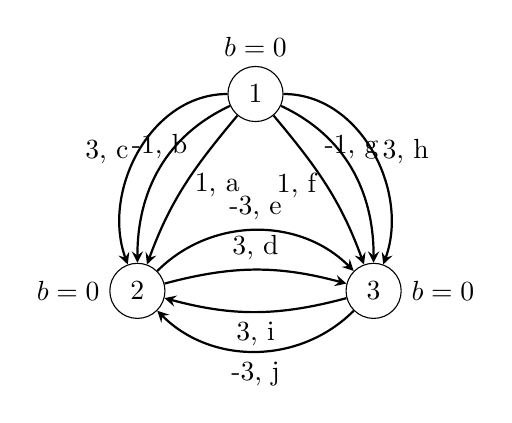
\begin{tikzpicture}[node distance=2.5 cm]
                        \node (1) [circleNode, label=above:{$b = 0$}] {1};
                        \node (2) [circleNode, below of=1, xshift=-1.5 cm, label=left:{$b = 0$}] {2};
                        \node (3) [circleNode, below of=1, xshift=1.5 cm, label=right:{$b = 0$}] {3};
                        \draw [arrow] (1) to [out = 230, in = 70] node [right] {1, a} (2);
                        \draw [arrow] (1) to [out = 205, in = 90] node [above] {-1, b} (2);
                        \draw [arrow] (1) to [out = 180, in = 110] node [left] {3, c} (2);
                        \draw [arrow] (1) to [out = 0, in = 70] node [right] {3, h} (3);
                        \draw [arrow] (1) to [out = -25, in = 90] node [above] {-1, g} (3);
                        \draw [arrow] (1) to [out = -50, in = 110] node [left] {1, f} (3);
                        \draw [arrow] (2) to [out = 15, in = 165] node [above] {3, d} (3);
                        \draw [arrow] (2) to [out = 45, in = 135] node [above] {-3, e} (3);
                        \draw [arrow] (3) to [out = -165, in = -15] node [below] {3, i} (2);
                        \draw [arrow] (3) to [out = -135, in = -45] node [below] {-3, j} (2);
                    \end{tikzpicture}
                \end{figure}

                Then for the following steps we can detect cycling:

                \begin{itemize}
                    \item $w(T, j) = w_j - w_i = -3 -3 = -6$, therefore $j$ in entering basis, $i$ is leaving basis.
                    \item $w(T, h) = w_h + w_j - w_a = 3-3-1=-1$, therefore $h$ is entering basis, $a$ is leaving basis.
                    \item $w(T, b) = w_b - w_j - w_h = -1 + 3 - 3 = -1$, therefore $b$ is entering basis, $j$ is leaving basis.
                    \item $w(T, d) = w_d - w_h + w_b = 3 - 3 - 1 = -1$, therefore $d$ is entering basis, $h$ is leaving basis.
                    \item $w(T, f) = w_f - w_d - w_b = 1 - 3 + 1 = -1$, therefore $f$ is entering basis, $b$ is leaving basis.
                    \item $w(T, e) = w_e - w_d = -3 -3 = -6$, therefore $e$ is entering basis, $d$ is leaving basis.
                    \item $w(T,c) = w_c + w_e - w_f = 3 -3 - 1 = -1$, therefore $c$ is entering basis, $f$ is leaving basis.
                    \item $w(T,g) = w_g - w_e - w_c = -1 + 3 - 3 = -1$, therefore $g$ is entering basis, $e$ is leaving basis.
                    \item $w(T,i) = w_i - w_c + w_g =3 - 3 - 1= -1 $, therefore $i$ is entering basis, $c$ is leaving basis.
                    \item $w(T,a) = w_a - w_i - w_g = 1 - 3 + 1 = -1$, therefore $a$ is entering basis, $g$ is leaving basis.                
                \end{itemize}

                \begin{figure}
                    \centering
                    \begin{subfigure}[c]{0.24\textwidth}
                        \centering
                        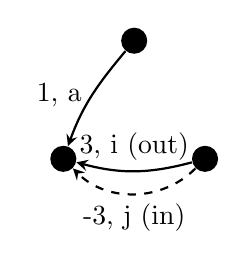
\begin{tikzpicture}[node distance=1.5 cm]
                            \node (1) [solidNode] {};
                            \node (2) [solidNode, below of = 1, xshift=-0.9 cm] {};
                            \node (3) [solidNode, below of = 1, xshift=0.9 cm] {};
                            \draw [arrow] (1) to [out = 230, in = 70] node [left] {1, a} (2);
                            \draw [arrow] (3) to [out = -165, in = -15] node [above] {3, i (out)} (2);
                            \draw [arrow, dashed] (3) to [out = -135, in = -45] node [below] {-3, j (in)} (2);
                        \end{tikzpicture}
                    \end{subfigure}
                    \qquad
                    \begin{subfigure}[c]{0.24\textwidth}
                        \centering
                        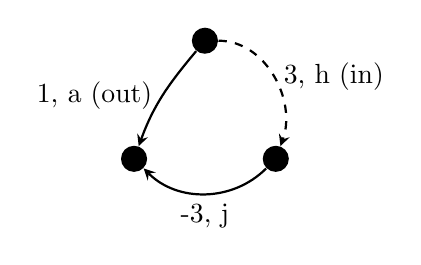
\begin{tikzpicture}[node distance=1.5 cm]
                            \node (1) [solidNode] {};
                            \node (2) [solidNode, below of = 1, xshift=-0.9 cm] {};
                            \node (3) [solidNode, below of = 1, xshift=0.9 cm] {};
                            \draw [arrow] (1) to [out = 230, in = 70] node [left] {1, a (out)} (2);
                            \draw [arrow] (3) to [out = -135, in = -45] node [below] {-3, j} (2);
                            \draw [arrow, dashed] (1) to [out = 0, in = 70] node [right] {3, h (in)} (3);
                        \end{tikzpicture}
                    \end{subfigure}
                    \qquad
                    \begin{subfigure}[c]{0.24\textwidth}
                        \centering
                        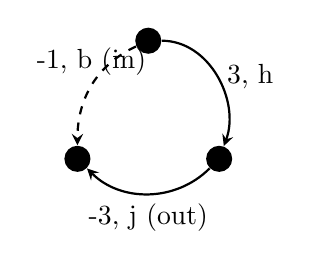
\begin{tikzpicture}[node distance=1.5 cm]
                            \node (1) [solidNode] {};
                            \node (2) [solidNode, below of = 1, xshift=-0.9 cm] {};
                            \node (3) [solidNode, below of = 1, xshift=0.9 cm] {};
                            \draw [arrow, dashed] (1) to [out = 205, in = 90] node [above] {-1, b (in)} (2);
                            \draw [arrow] (1) to [out = 0, in = 70] node [right] {3, h} (3);
                            \draw [arrow] (3) to [out = -135, in = -45] node [below] {-3, j (out)} (2);
                        \end{tikzpicture}
                    \end{subfigure}
                    \qquad
                    \begin{subfigure}[c]{0.24\textwidth}
                        \centering
                        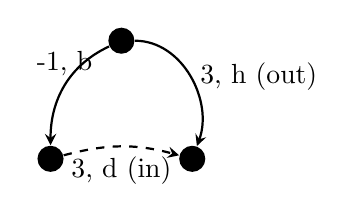
\begin{tikzpicture}[node distance=1.5 cm]
                            \node (1) [solidNode] {};
                            \node (2) [solidNode, below of = 1, xshift=-0.9 cm] {};
                            \node (3) [solidNode, below of = 1, xshift=0.9 cm] {};
                            \draw [arrow] (1) to [out = 205, in = 90] node [above] {-1, b} (2);
                            \draw [arrow] (1) to [out = 0, in = 70] node [right] {3, h (out)} (3);
                            \draw [arrow, dashed] (2) to [out = 15, in = 165] node [below] {3, d (in)} (3);
                        \end{tikzpicture}
                    \end{subfigure}
                    \qquad
                    \begin{subfigure}[c]{0.24\textwidth}
                        \centering
                        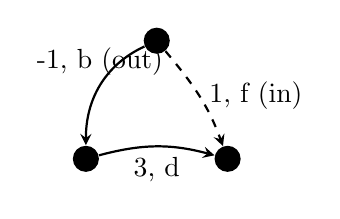
\begin{tikzpicture}[node distance=1.5 cm]
                            \node (1) [solidNode] {};
                            \node (2) [solidNode, below of = 1, xshift=-0.9 cm] {};
                            \node (3) [solidNode, below of = 1, xshift=0.9 cm] {};
                            \draw [arrow] (1) to [out = 205, in = 90] node [above] {-1, b (out)} (2);
                            \draw [arrow, dashed] (1) to [out = -50, in = 110] node [right] {1, f (in)} (3);
                            \draw [arrow] (2) to [out = 15, in = 165] node [below] {3, d} (3);
                        \end{tikzpicture}
                    \end{subfigure}
                    \qquad
                    \begin{subfigure}[c]{0.24\textwidth}
                        \centering
                        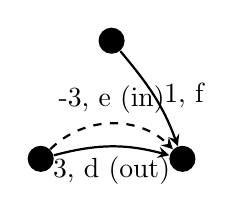
\begin{tikzpicture}[node distance=1.5 cm]
                            \node (1) [solidNode] {};
                            \node (2) [solidNode, below of = 1, xshift=-0.9 cm] {};
                            \node (3) [solidNode, below of = 1, xshift=0.9 cm] {};
                            \draw [arrow] (1) to [out = -50, in = 110] node [right] {1, f} (3);
                            \draw [arrow] (2) to [out = 15, in = 165] node [below] {3, d (out)} (3);
                            \draw [arrow, dashed] (2) to [out = 45, in = 135] node [above] {-3, e (in)} (3);
                        \end{tikzpicture}
                    \end{subfigure}
                    \qquad
                    \begin{subfigure}[c]{0.24\textwidth}
                        \centering
                        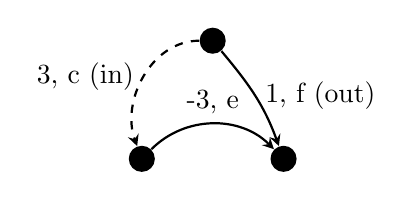
\begin{tikzpicture}[node distance=1.5 cm]
                            \node (1) [solidNode] {};
                            \node (2) [solidNode, below of = 1, xshift=-0.9 cm] {};
                            \node (3) [solidNode, below of = 1, xshift=0.9 cm] {};
                            \draw [arrow, dashed] (1) to [out = 180, in = 110] node [left] {3, c (in)} (2);
                            \draw [arrow] (1) to [out = -50, in = 110] node [right] {1, f (out)} (3);
                            \draw [arrow] (2) to [out = 45, in = 135] node [above] {-3, e} (3);
                        \end{tikzpicture}
                    \end{subfigure}
                    \qquad
                    \begin{subfigure}[c]{0.24\textwidth}
                        \centering
                        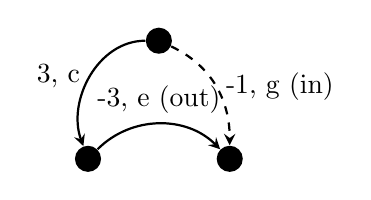
\begin{tikzpicture}[node distance=1.5 cm]
                            \node (1) [solidNode] {};
                            \node (2) [solidNode, below of = 1, xshift=-0.9 cm] {};
                            \node (3) [solidNode, below of = 1, xshift=0.9 cm] {};
                            \draw [arrow, dashed] (1) to [out = -25, in = 90] node [right] {-1, g (in)} (3);
                            \draw [arrow] (1) to [out = 180, in = 110] node [left] {3, c} (2);
                            \draw [arrow] (2) to [out = 45, in = 135] node [above] {-3, e (out)} (3);
                        \end{tikzpicture}
                    \end{subfigure}
                    \qquad
                    \begin{subfigure}[c]{0.24\textwidth}
                        \centering
                        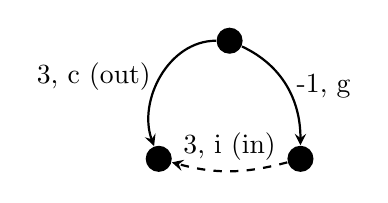
\begin{tikzpicture}[node distance=1.5 cm]
                            \node (1) [solidNode] {};
                            \node (2) [solidNode, below of = 1, xshift=-0.9 cm] {};
                            \node (3) [solidNode, below of = 1, xshift=0.9 cm] {};
                            \draw [arrow] (1) to [out = -25, in = 90] node [right] {-1, g} (3);
                            \draw [arrow] (1) to [out = 180, in = 110] node [left] {3, c (out)} (2);
                            \draw [arrow, dashed] (3) to [out = -165, in = -15] node [above] {3, i (in)} (2);
                        \end{tikzpicture}
                    \end{subfigure}
                    \qquad
                    \begin{subfigure}[c]{0.24\textwidth}
                        \centering
                        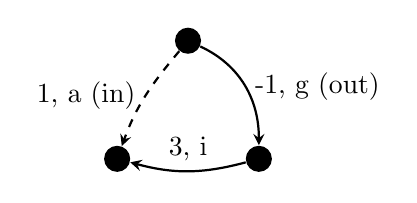
\begin{tikzpicture}[node distance=1.5 cm]
                            \node (1) [solidNode] {};
                            \node (2) [solidNode, below of = 1, xshift=-0.9 cm] {};
                            \node (3) [solidNode, below of = 1, xshift=0.9 cm] {};
                            \draw [arrow, dashed] (1) to [out = 230, in = 70] node [left] {1, a (in)} (2);
                            \draw [arrow] (1) to [out = -25, in = 90] node [right] {-1, g (out)} (3);
                            \draw [arrow] (3) to [out = -165, in = -15] node [above] {3, i} (2);
                        \end{tikzpicture}
                    \end{subfigure}
                    \qquad
                    \begin{subfigure}[c]{0.24\textwidth}
                        \centering
                        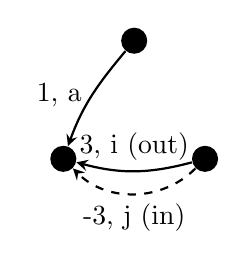
\begin{tikzpicture}[node distance=1.5 cm]
                            \node (1) [solidNode] {};
                            \node (2) [solidNode, below of = 1, xshift=-0.9 cm] {};
                            \node (3) [solidNode, below of = 1, xshift=0.9 cm] {};
                            \draw [arrow] (1) to [out = 230, in = 70] node [left] {1, a} (2);
                            \draw [arrow] (3) to [out = -165, in = -15] node [above] {3, i (out)} (2);
                            \draw [arrow, dashed] (3) to [out = -135, in = -45] node [below] {-3, j (in)} (2);
                        \end{tikzpicture}
                    \end{subfigure}
                \end{figure}

                The last graph is the same as the first graph, i.e., cycling detected.

            \paragraph{Cycling prevention}
                To Avoid cycling we will introduce the Modified Network Simplex Method. Let $T$ be a \textbf{rooted} spanning tree. Let $f$ be an arc in $T$, we say $f$ is \textbf{away} from the root $r$ if $t(f)$ is the component of $T-f$. Otherwise we say $f$ is \textbf{towards} $r$.

                Let $x$ be a feasible tree solution associated with $T$, then we say $T$ is a \textbf{strong feasible tree} if for every arc $f \in T$ with $x_f = 0$ then $f$ is away from $r\in T$.

                Modification to NSM:
                \begin{itemize}
                    \item The algorithm is initialed with a strong feasible tree.
                    \item $f$ in pivot phase is chosen to be the first reverse arc of $C(T, e)$ having $x_f = \theta$. By ``first'', we mean the first arc encountered in traversing $C(T, e)$ in the direction of $e$, starting at the vertex $i$ of $C(T, e)$ that minimizes the number of arcs in the unique $(r, i)$-path in $T$.
                \end{itemize}

                In the second rule above, $r$ could also be in the cycle, in that case, $i$ is $r$.

                Continue the previous example. Now should how we can avoid cycling:

                The first few (four) steps are the same as previous example, starting from

                \begin{figure}[H]
                    \centering
                    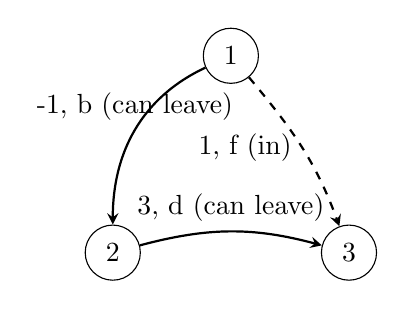
\begin{tikzpicture}[node distance=2.5 cm]
                        \node (1) [circleNode] {1};
                        \node (2) [circleNode, below of = 1, xshift=-1.5 cm] {2};
                        \node (3) [circleNode, below of = 1, xshift=1.5 cm] {3};
                        \draw [arrow] (1) to [out = 205, in = 90] node [above] {-1, b (can leave)} (2);
                        \draw [arrow, dashed] (1) to [out = -50, in = 110] node [left] {1, f (in)} (3);
                        \draw [arrow] (2) to [out = 15, in = 165] node [above] {3, d (can leave)} (3);
                    \end{tikzpicture}
                \end{figure}

                $w(T,f) = w_f - w_d - w_b = 1 - 3 + 1 = -1$. $f$ is entering basis, both $b$ and $d$ can leave the basis, according to the modified pivot rule, we choose the ``first'' arc encountered in traversing $C(T, e)$, which is $d$ to leave the basis, instead of $b$.

                \begin{figure}[H]
                    \centering
                    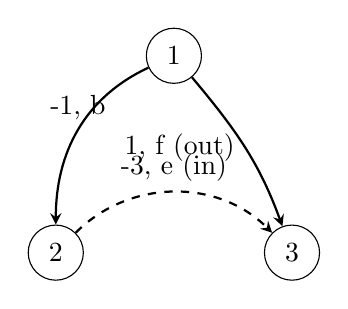
\begin{tikzpicture}[node distance=2.5 cm]
                        \node (1) [circleNode] {1};
                        \node (2) [circleNode, below of = 1, xshift=-1.5 cm] {2};
                        \node (3) [circleNode, below of = 1, xshift=1.5 cm] {3};
                        \draw [arrow] (1) to [out = 205, in = 90] node [above] {-1, b} (2);
                        \draw [arrow] (1) to [out = -50, in = 110] node [left] {1, f (out)} (3);
                        \draw [arrow, dashed] (2) to [out = 45, in = 135] node [above] {-3, e (in)} (3);
                    \end{tikzpicture}
                \end{figure}

                $w(T, e) = w_e - w_f + w_b = -5$, $e$ is entering basis, $f$ is leaving basis. Now the only arc to enter basis and maintain negative $w$ is $j$.

                \begin{figure}[H]
                    \centering
                    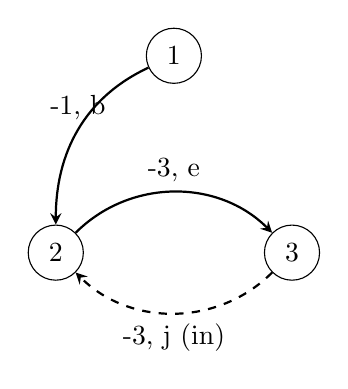
\begin{tikzpicture}[node distance=2.5 cm]
                        \node (1) [circleNode] {1};
                        \node (2) [circleNode, below of = 1, xshift=-1.5 cm] {2};
                        \node (3) [circleNode, below of = 1, xshift=1.5 cm] {3};
                        \draw [arrow] (1) to [out = 205, in = 90] node [above] {-1, b} (2);
                        \draw [arrow] (2) to [out = 45, in = 135] node [above] {-3, e} (3);
                        \draw [arrow, dashed] (3) to [out = -135, in = -45] node [below] {-3, j (in)} (2);
                    \end{tikzpicture}
                \end{figure}

                $w(T, j) = w_j + w_e = -6$, but in $C(T, j)$ there is no reversing arc, therefore we detect unboundness.

            \paragraph{Finding Initial Strong Feasible Tree}
                Pick a vertex in $D$ to be root $r$. The tree $T$ has an arc $e$ with the $t(e) = r$ and $h(e) = v$. For each $v\in V\setminus r$ with $b_v \ge 0$ and has an arc $e$ with $h(e) = r$ and $t(e) = v$ for each $v \in V\setminus r$ for which $b_v < 0$. Wherever possible the arcs of $T$ are chosen from $A$, where an appropriate arc doesn't exist. We create an \textbf{artificial arc} and give its weight $|V|(\max\{w_e: e\in A\}) + 1$. This is similar to Big-M method and if optimal solution contains artificial arcs ongoing arc problem is infeasible.

                Here is an example after adding artificial arcs:

                \begin{figure}[H]
                    \centering
                    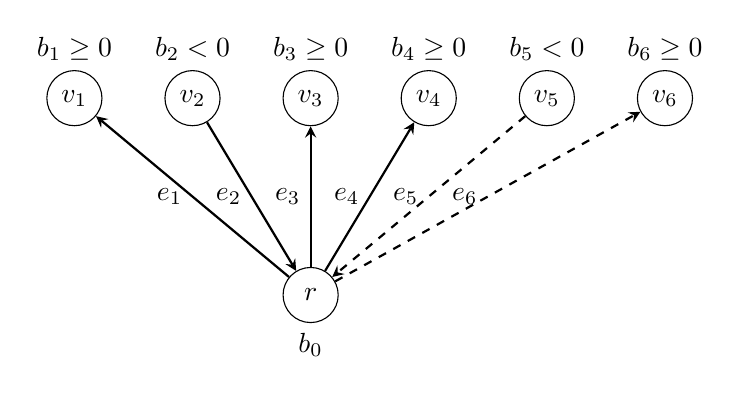
\begin{tikzpicture}[node distance = 1.5 cm]
                        \node (1) [circleNode, label=above:{$b_1 \ge 0$}] {$v_1$};
                        \node (2) [circleNode, label=above:{$b_2 < 0$}, right of = 1] {$v_2$};
                        \node (3) [circleNode, label=above:{$b_3 \ge 0$}, right of = 2] {$v_3$};
                        \node (4) [circleNode, label=above:{$b_4 \ge 0$}, right of = 3] {$v_4$};
                        \node (5) [circleNode, label=above:{$b_5 < 0$}, right of = 4] {$v_5$};
                        \node (6) [circleNode, label=above:{$b_6 \ge 0$}, right of = 5] {$v_6$};
                        \node (0) [circleNode, label=below:{$b_0$}, below of= 3, yshift=-1 cm] {$r$};
                        \draw [arrow] (0) -- node [left] {$e_1$} (1);
                        \draw [arrow] (2) -- node [left] {$e_2$} (0);
                        \draw [arrow] (0) -- node [left] {$e_3$} (3);
                        \draw [arrow] (0) -- node [left] {$e_4$} (4);
                        \draw [arrow, dashed] (5) -- node [left] {$e_5$} (0);
                        \draw [arrow, dashed] (0) -- node [left] {$e_6$} (6);
                    \end{tikzpicture}
                \end{figure}

                Where $e_5$ and $e_6$ are artificial arcs, the weight of those arcs are $|V|(\max\{w_e: e\in \mathcal{A}\}) + 1$. And the above tree is a basic feasible solution.

                We need to prove that such artificial arc has sufficiently large weight to guarantee

                \begin{itemize}
                    \item It will leave the basis, and
                    \item It will not enter the basis again (for this, just delete the artificial arc after it leaves the basis, then it will never enter the basis again)
                \end{itemize}

                \begin{proof}
                    Now prove that such arcs will always leave the basis. Before the prove we give some notation. 
                    \begin{itemize}
                        \item Define set $E$ as the set of arcs which is not artificial arc, in the above example, $E = \{e_1, e_2, e_3, e_4\}$. 
                        \item Define set $A$ as the set of arcs which are artificial arcs, in the above example, $A = \{e_5, e_6\}$. Noticed that $E \cap A = \emptyset$.
                        \item Define set $M$ as the vertices in the spanning tree that is reachable from $r$ by $E$, in the above example, $M = \{v_1, v_2, v_3, v_4\}$.
                        \item Define $M^\prime = (V\setminus r) \setminus M$ in the tree that can only be reached from $r$ by $A$, i.e., artificial arcs, in the above example, $M^\prime = \{v_5, v_6\}$. 
                    \end{itemize}

                    Then the initial basic feasible solution is a graph 
                    \begin{equation*}
                        G_0 = <M\cup M^\prime \cup \{r\}, E\cup A>
                    \end{equation*}
                    Denote the origin graph 
                    \begin{equation*}
                        G = <V, \mathcal{A}>
                    \end{equation*}
                    Notice that with the artificial arcs, $G_0$ is not a subgraph of $G$.

                    Let $(M\cup\{r\}, M^\prime)$ be a cut in the origin graph $G$. For the vertices in $M^\prime$, one of the following cases will happen:
                    \begin{itemize}
                        \item case 1: $\sum_{v \in M^\prime} b_v \ge 0$
                        \item case 2: $\sum_{v \in M^\prime} b_v < 0$
                    \end{itemize}

                    For case 1, we claim that at least one of the vertices $v_{M^\prime} \in M^\prime$ with $b_{v_{M^\prime}} \ge 0$ linked by an arc, say $f$, such that $h(f) = v_{M^\prime}$ and $t(f) = v_M \in M$. Otherwise the balance of flow cannot hold in the origin graph $G$. Furthermore, denote the artificial arc from $r$ to $v_{M^\prime}$ by $e_{rv_{M^\prime}}$.

                    Notice that for $v_M$ there is not necessarily be an arc between $r$ and $v_M$, but there must exists an $(r, v_M)$-path denoted by $P$, for $M$ is the set of vertices that reachable from $r$ by arcs in $E$.

                    Take that arc $f$ as entering arc to the basis. Then 
                    \begin{equation*}
                        C(T, f) = re_{rv_{M^\prime}}v_{M^\prime}fv_MPr
                    \end{equation*}
                    For
                    \begin{equation*}
                        w(T, f) = w_f - w_{e_{rv_{M^\prime}}} + \sum_{e \in P} d_e w_e
                    \end{equation*}
                    where $d_e = 1$ if $w_e$ is forward in $P$ and $d_e = -1$ otherwise.

                    Now that $w_{e_{rv_{M^\prime}}} = |V|(\max\{w_e: e\in \mathcal{A}\}) + 1$, it guarantees that
                    \begin{align*}
                        w(T, f) &= w_f + \sum_{e \in P} d_e w_e - w_{e_{rv_{M^\prime}}}\\
                                &\le w_f + \sum_{e \in P}w_e - w_{e_{rv_{M^\prime}}}\\
                                &\le \sum_{e \in \mathcal{A}}w_e - w_{e_{rv_{M^\prime}}}\\
                                &\le |V|(\max\{w_e: e\in \mathcal{A}\}) - w_{e_{rv_{M^\prime}}}\\
                                &\le -1 < 0 
                    \end{align*}
                    So $f$ can enter the basis, and the artificial variable $e_{rv_{M^\prime}}$ will leave the basis, for it is the most violated reverse arc in the $C(T, f)$. When we put $f$ into the basis, update $G_0$, such that $M \leftarrow M \cup \{v_{M^\prime}\}$ and $M^\prime \leftarrow M^\prime \setminus \{v_{M^\prime}\}$.

                    For case 2, it is similar. At least one of the vertices $v_{M^\prime} \in M^\prime$ with $b_{v_{M^\prime}} < 0$ linked by an arc, say $f\prime$, such that $t(f^\prime) = v_{M^\prime}$ and $h(f^\prime) = v_M \in M$. Otherwise the balance of flow cannot hold in the origin graph $G$. Furthermore, denote the artificial arc from $v_{M^\prime}$ to $r$ by $e_{v_{M^\prime}r}$.

                    Similarly we can find a cycle $C(T, f^\prime) = rP^\prime v_M f^\prime v_{M^\prime}e_{v_{M^\prime}r}r$. $w(T, f^\prime) = w_{f^\prime} - w_{e_{rv_{M^\prime}}} + \sum_{e \in P^\prime} d_e w_e$, where $d_e = 1$ if $w_e$ is forward in $P\prime$ and $d_e = -1$. We can prove $w(T, f^\prime) \le -1 < 0$. That that $f^\prime$ as entering arc to the basis, similarly move $v_{M^\prime}$ form set $M^\prime$ to $M$.

                    The above case can be dealt with iteratively until set $M^\prime$ become $\emptyset$, at which stage there is no artificial arc in the basic feasible solution. Which means all the artificial variable can leave the basis.
                \end{proof}

        % \subsection{Out-of-Kilter algorithm}
        %     This algorithm is a Primal-dual method and is applied to the minimum weight circulation problem.

        %     For LP optimality conditions we need primal feasibility, dual feasibility and complementary slackness, i.e., KKT conditions. Primal and dual feasibility are obvious so we need to show complementary slackness through following theorem.

        %     \begin{theorem}
        %         Let $x$ be a feasible circulation flow for $(D, l, u, w)$. And suppose there exists a real value vector $\{y_i: i \in V\}$ which we called \textbf{vertex-numbers}. For all edges $e\in A$
        %         \begin{align*}
        %             y_{h(e)} - y_{t(e)} &> w_e \text{ implies } x_e = u_e\\
        %             y_{h(e)} - y_{t(e)} &< w_e \text{ implies } x_e = l_e
        %         \end{align*}
        %         Then $x$ is optimal to the circulation problem.
        %     \end{theorem}

        %     \begin{proof}
        %         For each $e \in A$ define
        %         \begin{align*}
        %             \gamma_e &= \max\{y_{h(e)} - y_{t(e)} - w_e, 0\} \\
        %             \mu_e &= \max\{w_e - y_{h(e)} + y_{t(e)}, 0\}
        %         \end{align*}
        %         Then
        %         \begin{equation*}
        %             \gamma_e - \mu_e = y_{h(e)} - y_{t(e)} - w_e
        %         \end{equation*}
        %         Furthermore
        %         \begin{align*}
        %             &\sum_{e\in A} (\mu_el_e - \gamma_eu_e) \\
        %             &= \sum_{e\in A} (\mu_el_e - \gamma_eu_e) + \sum_{i \in V}y_i(\sum_{h(e) = i} x_e - \sum_{t(e) = i} x_e)\\
        %             &= \sum_{e\in A} (\mu_el_e - \gamma_eu_e + x_e(y_{h(e)} - y_{t(e)}))\\
        %             &= \sum_{e\in A} (\mu_el_e - \gamma_eu_e + x_e(\gamma_e - \mu_e + w_e))\\
        %             &= \sum_{e\in A} (\gamma_e(x_e - u_e) + \mu_e(l_e - x_e) + x_ew_e)\\
        %             &\le \sum_{e\in A} x_ew_e 
        %         \end{align*}
        %         The last inequality will be satisfied as equality iff the first two hold.
        %     \end{proof}

        %     The following is the formulation of circulation problem
        %     \begin{align*}
        %         \text{(P)} \quad \min \quad & wx\\
        %         \text{s.t.} \quad & Nx = 0 \quad y \\
        %                           & x \ge l \quad z^l \\
        %                           & -x \le -u \quad z^u\\
        %         \text{(D)} \quad \max \quad & lz^l - uz^u \\
        %         \text{(s.t.)} \quad & yN^{-1} + z^l-z^u \le w\\
        %                             & y \quad free\\
        %                             &z^l, z^u \ge 0 \\
        %         \text{(CS)} \quad & y_{h(e)} - y_{t(e)} > w_e \Rightarrow x_e = u_e\\
        %                           & y_{h(e)} - y_{t(e)} < w_e \Rightarrow x_e = l_e
        %     \end{align*}

        %     There is an alternative way of circulation optimality for a circulation problem. We define a \textbf{kilter-diagram} as follows.

        %     For every edge construct the following:
        %     \begin{figure}[H]
        %         \centering
        %         \begin{tikzpicture}
        %             \draw [arrow] (0, 0) -- (0, 3);
        %             \draw [arrow] (0, 0) -- (3, 0);
        %             \draw [link, line width=0.6 mm] (1, -1) -- (1, 1) -- (2, 1) -- (2, 3);
        %             \draw node at (0, 3) [above] {$y_{h(e)} - y_{t(e)}$};
        %             \draw node at (3, 0) [above] {$x_e$};
        %             \draw node at (1, -0.5) [left] {$l_e$};
        %             \draw node at (2, 0) [above] {$u_e$};
        %             \draw node at (0, 1) [left] {$w_e$};
        %         \end{tikzpicture}
        %     \end{figure}

        %     For each point $(x_e, y_{h(e)} - y_{t(e)})$ we define a \textbf{kilter-number} $k_e$, be the minimum positive distance change in $x_e$ required to put in on the kilter line.
        %     \begin{example}
        %         For edge $e: w_e = 2, l_e = 0, u_e = 3$, assume $x_e = 2, y_{h(e)} - y_{t(e)} = 3$, then $k_e = 1$
        %     \end{example}

        %     \begin{figure}[H]
        %         \centering
        %         \begin{tikzpicture}
        %             \draw [arrow] (0, 0) -- (0, 4);
        %             \draw [arrow] (0, 0) -- (4, 0);
        %             \draw [link, line width=0.6 mm] (0, -1) -- (0, 2) -- (3, 2) -- (3, 4);
        %             \draw node at (0, 4) [above] {$y_{h(e)} - y_{t(e)}$};
        %             \draw node at (4, 0) [above] {$x_e$};
        %             \draw node at (0, -0.5) [left] {0};
        %             \draw node at (3, 0) [above] {3};
        %             \draw node at (0, 2) [left] {2};
        %             \fill (2, 3) circle [radius=2 pt];
        %             \draw node at (2, 3) [above, xshift=-0.6 cm] {$(x_e, y_{h(e)} - y_{t(e)})$};
        %             \draw node at (2, 3) [below] {(2, 3)};
        %             \draw [link, dashed] (2, 3) -- (3, 3);
        %         \end{tikzpicture}
        %     \end{figure}

        %     \begin{lemma}
        %         If for every circulation $x$ and vertex number $y$ we have $\sum_{e \in A} k_e = 0$, then $x$ is optimal.
        %     \end{lemma}

        %     \begin{proof}
        %         Since $k_e$ is a nonnegative number, then the only way that $\sum_{e \in A} k_e = 0$ is $k_e = 0, \forall e\in A$, which means $\forall e\in A, l_e \le x_e \le u_e$. Furthermore, the complementary slackness are satisfied.
        %     \end{proof}

        %     General idea of algorithm is as follows. Suppose we are given a circulation $x$ and vertex-numbers $y$ (we do not require feasibility). Usually we pick $x=0, y=0$. If every edge is in kilter-line then we are optimal.

        %     Otherwise there is at least one edge $e^*$ that is out-of kilter. The algorithm consist of two phases, one called \textbf{flow-change} phase (horizontally), then other \textbf{number-change} phase (vertically).

        %     In the flow-change phase, we want to find a new circulation for an out-of-kilter edge $e^*$ say $\hat{e}$ such that we reduce the kilter number $k_{e^*}$, without increasing any other kilter number for other edges.

        %     To do this, denote the edges of $e^*$ to be $s$ and $t$, where such that $k_{e^*}$ will be decreased by increasing the flow from $s$ to $t$ on $e^*$.

        %     If $e^*=(s, t)$ this will accomplished by increasing $x_{e^*}$ and if $e=(t, s)$ it is accomplished by decreasing $x_{e^*}$. 

        %     To do this we look for an $(s, t)$-path $p$ of the following edges.

        %     \begin{itemize}
        %         \item If $e$ is forward in $p$, then increasing $x_e$ does not increase $k_e$ and
        %         \item If $e$ is reversed in $p$, then decreasing $x_e$ dose not increase $k_e$
        %     \end{itemize}

        %     In terms of kilter diagram, an arc satisfies ``forward'' if it is forward and in left side of kilter line, and it satisfies ``reversed'' if it is reverse and in right side of kilter line.

        %     Suppose we can not find such a path. From $s$ to $t$, let $x$ be the vertices that can decrease by an augmenting path. Then either we can change the vertex numbers $y$ so that $\sum_{e\in A} k_e$ does not increase but $x$ does, or we can show that problem is infeasible.

        %     The sketch of Out-of-kilter algorithm is as follows:
        %     \begin{itemize}
        %         \item \textbf{INPUT} a minimum circulation problem $(D, l, u, w)$ a circulation $x$ and vertex-numbers $y$
        %         \item \textbf{OUTPUT} conclusion that $(D, l, u, w)$ is infeasible or an minimum weighted flow.
        %         \item Step 1: If every arc is in kilter $(k_e = 0, \forall e\in A)$. Stop with $x$ is optimal. Otherwise let $e^*$ be an out-of-kilter arc. If increasing $x_{e^*}$ decreases $k_{e^*}$ set $s=h(e^*)$ and $t(e^*)$ otherwise set $s=t(e^*)$ and $t=h(e^*)$
        %         \item Step 2: If there exists an $(s, t)$ augmenting path $p$ then goto Step 3, otherwise goto Step 4.
        %         \item Step 3: Set $y_e = y_{h(e)} - y_{t(e)}, e\in A$
        %         $\begin{cases}
        %             \Delta_1 &= \min\{u_e - x_e: e \text{ is forward and } y_e \ge w_e\}\\
        %             \Delta_2 &= \min\{l_e - x_e: e \text{ is forward and } y_e < w_e\}\\
        %             \Delta_3 &= \min\{x_e - l_e: e \text{ is reverse and } y_e \le w_e\}\\
        %             \Delta_4 &= \min\{x_e - u_e: e \text{ is reverse and } y_e > w_e\}
        %         \end{cases}$\\
        %         and $\Delta = \min\{\Delta_i, i = 1, 2, 3, 4\}$. Increase $x_e$ by $\Delta$ on each forward arc in $p$, decrease $x_e$ by $\Delta$ on each reverse arc in $p$.\\
        %         If $e^* = (s, t)$ decrease $x_{e^*}$ by $\Delta$, otherwise increase $x_{e^*}$ by $\Delta$\\
        %         If $k_{e^*} > 0$ goto Step 2. otherwise goto Step 1.
        %         \item Step 4: Let $X$ be the set of vertices reachable from $s$ by augmenting paths, then $t \notin X$, if every arc $e$ with $h(e) \in X$ has $x_e \le l_e$ and every arc $e$ with $t(e) \in X$ has $x_e \ge u_e$, and at least one of the above inequality is strict, then Stop with problem infeasible. Otherwise set
        %             $\delta_1 = \min\{w_e - y_e: t(e) \in X, y_e < w_e, x_e \le u_e \neq l_e\}$
        %             $\delta_2 = \min\{y_e - w_e: h(e) \in X, y_e > w_e, x_e \ge u_e \neq l_e\}$
        %             $\delta = \min\{\delta_1, \delta_2\}$
        %         Set $y_i = y_i + \delta$ for $i \notin X$. If $k_{e^*} > 0$, goto Step 2, otherwise goto Step 1.
        %     \end{itemize}                

        %     Out-of-kilter takes $O(|E||V|K)$ where $K = \sum_{e\in A} k_e$. However, there is an algorithm called \textbf{scaling algorithm} that uses out-of-kilter as subroutine that runs in $O(R|E|^2|V|)$ where $R = \lceil \max\{\log_2 u_e: e\in A\}\rceil$

    % \bibliography{literature}
\end{document}